%% authorvak
\nocite{Sinuk2020}%
\nocite{Karatach2021}%
\nocite{Karatach2023}%
\nocite{vakbib4}%
\nocite{vakbib5}%
\nocite{vakbib6}%
\nocite{vakbib7}%
\nocite{vakbib8}%
\nocite{vakbib9}%
\nocite{vakbib10}%
\nocite{vakbib11}%
\nocite{vakbib12}%
%
%% authorwos
\nocite{Sinuk2023}%
\nocite{Karatach2024}%
\nocite{wosbib1}%
%
%% authorscopus
\nocite{Karatach2023b}%
%
%% authorpatent
\nocite{patbib1}%
%
%% authorconf
\nocite{Karatach2020}%
\nocite{Karatach2021parallel}%
\nocite{Sinuk2022}%
\nocite{Karatach2022}%
\nocite{Sinuk2023kii}%
%
%% authorother
\nocite{bib1}%
\nocite{bib2}%
%
%% authorprogram
\nocite{Rospatent1}%
\nocite{Rospatent2}%

\pdfbookmark{Общая характеристика работы}{characteristic}             % Закладка pdf
\section*{Общая характеристика работы}

\newcommand{\actuality}{\pdfbookmark[1]{Актуальность}{actuality}\underline{\textbf{\actualityTXT}}}
\newcommand{\progress}{\pdfbookmark[1]{Разработанность темы}{progress}\underline{\textbf{\progressTXT}}}
\newcommand{\aim}{\pdfbookmark[1]{Цели}{aim}\underline{{\textbf\aimTXT}}}
\newcommand{\tasks}{\pdfbookmark[1]{Задачи}{tasks}\underline{\textbf{\tasksTXT}}}
\newcommand{\aimtasks}{\pdfbookmark[1]{Цели и задачи}{aimtasks}\aimtasksTXT}
\newcommand{\researchObject}{\pdfbookmark[1]{Объект исследования}{researchObject}\underline{\textbf{\researchObjectTXT}}}
\newcommand{\researchSubject}{\pdfbookmark[1]{Предмет исследования}{researchSubject}\underline{\textbf{\researchSubjectTXT}}}
\newcommand{\novelty}{\pdfbookmark[1]{Научная новизна}{novelty}\underline{\textbf{\noveltyTXT}}}
\newcommand{\theoreticalValue}{\pdfbookmark[1]{Теоретическая значимость}{theoreticalValue}\underline{\textbf{\theoreticalValueTXT}}}
\newcommand{\practicalValue}{\pdfbookmark[1]{Практическая значимость}{practicalValue}\underline{\textbf{\practicalValueTXT}}}
\newcommand{\influence}{\pdfbookmark[1]{Практическая значимость}{influence}\underline{\textbf{\influenceTXT}}}
\newcommand{\methods}{\pdfbookmark[1]{Методология и методы исследования}{methods}\underline{\textbf{\methodsTXT}}}
\newcommand{\defpositions}{\pdfbookmark[1]{Положения, выносимые на защиту}{defpositions}\underline{\textbf{\defpositionsTXT}}}
\newcommand{\specialityRelation}{\pdfbookmark[1]{Область исследования}{specialityRelation}\underline{\textbf{\specialityRelationTXT}}}
\newcommand{\reliability}{\pdfbookmark[1]{Достоверность}{reliability}\underline{\textbf{\reliabilityTXT}}}
\newcommand{\probation}{\pdfbookmark[1]{Апробация}{probation}\underline{\textbf{\probationTXT}}}
\newcommand{\contribution}{\pdfbookmark[1]{Личный вклад}{contribution}\underline{\textbf{\contributionTXT}}}
\newcommand{\publications}{\pdfbookmark[1]{Публикации}{publications}\underline{\textbf{\publicationsTXT}}}


{\actuality} Обзор, введение в тему, обозначение места данной работы в
мировых исследованиях и~т.\:п., можно использовать ссылки на~другие
работы~\autocite{Gosele1999161,Lermontov}
(если их~нет, то~в~автореферате
автоматически пропадёт раздел <<Список литературы>>). Внимание! Ссылки
на~другие работы в~разделе общей характеристики работы можно
использовать только при использовании \verb!biblatex! (из-за технических
ограничений \verb!bibtex8!. Это связано с тем, что одна
и~та~же~характеристика используются и~в~тексте диссертации, и в
автореферате. В~последнем, согласно ГОСТ, должен присутствовать список
работ автора по~теме диссертации, а~\verb!bibtex8! не~умеет выводить в~одном
файле два списка литературы).
При использовании \verb!biblatex! возможно использование исключительно
в~автореферате подстрочных ссылок
для других работ командой \verb!\autocite!~\autocite{Marketing}, а~также цитирование
собственных работ командой \verb!\cite!. Для этого в~файле
\verb!common/setup.tex! необходимо присвоить положительное значение
счётчику \verb!\setcounter{usefootcite}{1}!.

Для генерации содержимого титульного листа автореферата, диссертации
и~презентации используются данные из файла \verb!common/data.tex!. Если,
например, вы меняете название диссертации, то оно автоматически
появится в~итоговых файлах после очередного запуска \LaTeX. Согласно
ГОСТ 7.0.11-2011 <<5.1.1 Титульный лист является первой страницей
диссертации, служит источником информации, необходимой для обработки и
поиска документа>>. Наличие логотипа организации на~титульном листе
упрощает обработку и~поиск, для этого разметите логотип вашей
организации в папке images в~формате PDF (лучше найти его в векторном
варианте, чтобы он хорошо смотрелся при печати) под именем
\verb!logo.pdf!. Настроить размер изображения с логотипом можно
в~соответствующих местах файлов \verb!title.tex!  отдельно для
диссертации и автореферата. Если вам логотип не~нужен, то просто
удалите файл с~логотипом.

\ifsynopsis
Этот абзац появляется только в~автореферате.
Для формирования блоков, которые будут обрабатываться только в~автореферате,
заведена проверка условия \verb!\!\verb!ifsynopsis!.
Значение условия задаётся в~основном файле документа (\verb!synopsis.tex! для
автореферата).
\else
Этот абзац появляется только в~диссертации.
Через проверку условия \verb!\!\verb!ifsynopsis!, задаваемого в~основном файле
документа (\verb!dissertation.tex! для диссертации), можно сделать новую
команду, обеспечивающую появление цитаты в~диссертации, но~не~в~автореферате.
\fi

% {\progress}
% Этот раздел должен быть отдельным структурным элементом по
% ГОСТ, но он, как правило, включается в описание актуальности
% темы. Нужен он отдельным структурынм элемементом или нет ---
% смотрите другие диссертации вашего совета, скорее всего не нужен.

{\aim} данной работы является повышение эффективности анализа неопределенных данных путем разработки математического и программного обеспечения на основе мягких вычислений.

Для~достижения поставленной цели необходимо было решить следующие {\tasks}:
\begin{enumerate}[beginpenalty=10000] % https://tex.stackexchange.com/a/476052/104425
  \item Провести обзор проблем и предлагаемых подходов построения нечетких систем анализа данных с качественным описанием.
  \item Разработать метод вывода на основое нечеткого значения истинности для системы MISO-сструктуры логического типа, обеспечивающий полиномиальную вычислительную сложность.
  \item Выполнить программную реализацию выработанного метода нечеткого вывода с использованием технологии параллельных вычислений CUDA, обеспечив эффективность реализации за счет внедрения оптимизаций алгоритма вывода.
  \item Применить разработанный модуль нечеткого логического вывода для высокопроизводительного анализа зашумленных данных в выбранной предметной области.
\end{enumerate}


{\novelty}
\begin{enumerate}[beginpenalty=10000] % https://tex.stackexchange.com/a/476052/104425
  \item Впервые применено нечеткое значение истинности и принцип обобщения для получения выходного значения при нескольких нечетких входах в соответствии с обобщенным нечетким правилом вывода \textit{modus ponens} для нечетких систем логического типа, в результате чего была получена новая структура базы правил: <<Если \textit{истинно}, то $B_k$>>.
  \item Разработан метод нечеткого вывода логического типа с использованием нечеткого значения истинности, имеющий полиномиальную вычислительную сложность при многих нечетких входах.
  \item Разработан метод регрессии временных рядов с нечеткими оценками измеренных значений на основе предложенного метода нечеткого вывода логического типа и алгоритм построения базы правил \dots.
  \item Разработан параллельный алгоритм, реализующий нечеткий вывод на основе нечеткого значения истинности с применением отбора \dots
\end{enumerate}

{\influence} \ldots

{\methods} \ldots

{\defpositions}
\begin{enumerate}[beginpenalty=10000] % https://tex.stackexchange.com/a/476052/104425
  \item Метод вывода для нечетких систем логического типа на основе нечеткого значения истинности, имеющий полиномиальную вычислительную сложность при многих нечетких входах.
  \item Метод регрессии для временных рядов с нечеткими оценками измеренных значений на основе метода нечеткого вывода логического типа.
  \item Разработанный вид нечетких правил <<Если \textit{истинно}, то $B_k$>>.
  \item Разработанный параллельный алгоритм для предложенного метода вывода и его эффективная реализация на графическом процессоре с поддержкой технологии CUDA.
  \item \dots
  \item \dots
\end{enumerate}
В папке Documents можно ознакомиться с решением совета из Томского~ГУ
(в~файле \verb+Def_positions.pdf+), где обоснованно даются рекомендации
по~формулировкам защищаемых положений.

\textbf{Соответствие диссертации научной специальности.} Диссертационная работа соответствует паспорту специальности 2.3.1. <<Системный анализ, управление и обработка информации, статистика>> по следующим областям исследования:
\begin{itemize}
  \item п. 10 <<Методы и алгоритмы интеллектуальной поддержки при принятии управленческих решений в технических системах>>.
\end{itemize}


{\reliability} полученных результатов обеспечивается \ldots \ Результаты находятся в соответствии с результатами, полученными другими авторами.

{\probation}
Основные результаты работы докладывались~на:
перечисление основных конференций, симпозиумов и~т.\:п.

{\contribution} Все изложенные в диссертации результаты исследования получены либо соискателем лично, либо при его непосредственном участии.

\ifnumequal{\value{bibliosel}}{0}
{%%% Встроенная реализация с загрузкой файла через движок bibtex8. (При желании, внутри можно использовать обычные ссылки, наподобие `\cite{vakbib1,vakbib2}`).
    {\publications} Основные результаты по теме диссертации изложены
    в~XX~печатных изданиях,
    X из которых изданы в журналах, рекомендованных ВАК,
    X "--- в тезисах докладов.
}%
{%%% Реализация пакетом biblatex через движок biber
    \begin{refsection}[bl-author, bl-registered]
        % Это refsection=1.
        % Процитированные здесь работы:
        %  * подсчитываются, для автоматического составления фразы "Основные результаты ..."
        %  * попадают в авторскую библиографию, при usefootcite==0 и стиле `\insertbiblioauthor` или `\insertbiblioauthorgrouped`
        %  * нумеруются там в зависимости от порядка команд `\printbibliography` в этом разделе.
        %  * при использовании `\insertbiblioauthorgrouped`, порядок команд `\printbibliography` в нём должен быть тем же (см. biblio/biblatex.tex)
        %
        % Невидимый библиографический список для подсчёта количества публикаций:
        \phantom{\printbibliography[heading=nobibheading, section=1, env=countauthorvak,          keyword=biblioauthorvak]%
        \printbibliography[heading=nobibheading, section=1, env=countauthorwos,          keyword=biblioauthorwos]%
        \printbibliography[heading=nobibheading, section=1, env=countauthorscopus,       keyword=biblioauthorscopus]%
        \printbibliography[heading=nobibheading, section=1, env=countauthorconf,         keyword=biblioauthorconf]%
        \printbibliography[heading=nobibheading, section=1, env=countauthorother,        keyword=biblioauthorother]%
        \printbibliography[heading=nobibheading, section=1, env=countregistered,         keyword=biblioregistered]%
        \printbibliography[heading=nobibheading, section=1, env=countauthorpatent,       keyword=biblioauthorpatent]%
        \printbibliography[heading=nobibheading, section=1, env=countauthorprogram,      keyword=biblioauthorprogram]%
        \printbibliography[heading=nobibheading, section=1, env=countauthor,             keyword=biblioauthor]%
        \printbibliography[heading=nobibheading, section=1, env=countauthorvakscopuswos, filter=vakscopuswos]%
        \printbibliography[heading=nobibheading, section=1, env=countauthorscopuswos,    filter=scopuswos]}%
        %
        \nocite{*}%
        %
        {\publications} Основные результаты по теме диссертации изложены в~\arabic{citeauthor}~печатных изданиях,
        \arabic{citeauthorvak} из которых изданы в журналах, рекомендованных ВАК%
        \ifnum \value{citeauthorscopuswos}>0%
            , \arabic{citeauthorscopuswos} "--- в~периодических научных журналах, индексируемых Web of~Science и Scopus%
        \fi%
        \ifnum \value{citeauthorconf}>0%
            , \arabic{citeauthorconf} "--- в~тезисах докладов.
        \else%
            .
        \fi%
        \ifnum \value{citeregistered}=1%
            \ifnum \value{citeauthorpatent}=1%
                Зарегистрирован \arabic{citeauthorpatent} патент.
            \fi%
            \ifnum \value{citeauthorprogram}=1%
                Зарегистрирована \arabic{citeauthorprogram} программа для ЭВМ.
            \fi%
        \fi%
        \ifnum \value{citeregistered}>1%
            Зарегистрированы\ %
            \ifnum \value{citeauthorpatent}>0%
            \formbytotal{citeauthorpatent}{патент}{}{а}{}%
            \ifnum \value{citeauthorprogram}=0 . \else \ и~\fi%
            \fi%
            \ifnum \value{citeauthorprogram}>0%
            \formbytotal{citeauthorprogram}{программ}{а}{ы}{} для ЭВМ.
            \fi%
        \fi%
        % К публикациям, в которых излагаются основные научные результаты диссертации на соискание учёной
        % степени, в рецензируемых изданиях приравниваются патенты на изобретения, патенты (свидетельства) на
        % полезную модель, патенты на промышленный образец, патенты на селекционные достижения, свидетельства
        % на программу для электронных вычислительных машин, базу данных, топологию интегральных микросхем,
        % зарегистрированные в установленном порядке.(в ред. Постановления Правительства РФ от 21.04.2016 N 335)
    \end{refsection}%
    \begin{refsection}[bl-author, bl-registered]
        % Это refsection=2.
        % Процитированные здесь работы:
        %  * попадают в авторскую библиографию, при usefootcite==0 и стиле `\insertbiblioauthorimportant`.
        %  * ни на что не влияют в противном случае
        \nocite{vakbib2}%vak
        \nocite{patbib1}%patent
        \nocite{progbib1}%program
        \nocite{bib1}%other
        \nocite{confbib1}%conf
    \end{refsection}%
        %
        % Всё, что вне этих двух refsection, это refsection=0,
        %  * для диссертации - это нормальные ссылки, попадающие в обычную библиографию
        %  * для автореферата:
        %     * при usefootcite==0, ссылка корректно сработает только для источника из `external.bib`. Для своих работ --- напечатает "[0]" (и даже Warning не вылезет).
        %     * при usefootcite==1, ссылка сработает нормально. В авторской библиографии будут только процитированные в refsection=0 работы.
}

При использовании пакета \verb!biblatex! будут подсчитаны все работы, добавленные
в файл \verb!biblio/author.bib!. Для правильного подсчёта работ в~различных
системах цитирования требуется использовать поля:
\begin{itemize}
        \item \texttt{authorvak} если публикация индексирована ВАК,
        \item \texttt{authorscopus} если публикация индексирована Scopus,
        \item \texttt{authorwos} если публикация индексирована Web of Science,
        \item \texttt{authorconf} для докладов конференций,
        \item \texttt{authorpatent} для патентов,
        \item \texttt{authorprogram} для зарегистрированных программ для ЭВМ,
        \item \texttt{authorother} для других публикаций.
\end{itemize}
Для подсчёта используются счётчики:
\begin{itemize}
        \item \texttt{citeauthorvak} для работ, индексируемых ВАК,
        \item \texttt{citeauthorscopus} для работ, индексируемых Scopus,
        \item \texttt{citeauthorwos} для работ, индексируемых Web of Science,
        \item \texttt{citeauthorvakscopuswos} для работ, индексируемых одной из трёх баз,
        \item \texttt{citeauthorscopuswos} для работ, индексируемых Scopus или Web of~Science,
        \item \texttt{citeauthorconf} для докладов на конференциях,
        \item \texttt{citeauthorother} для остальных работ,
        \item \texttt{citeauthorpatent} для патентов,
        \item \texttt{citeauthorprogram} для зарегистрированных программ для ЭВМ,
        \item \texttt{citeauthor} для суммарного количества работ.
\end{itemize}
% Счётчик \texttt{citeexternal} используется для подсчёта процитированных публикаций;
% \texttt{citeregistered} "--- для подсчёта суммарного количества патентов и программ для ЭВМ.

Для добавления в список публикаций автора работ, которые не были процитированы в
автореферате, требуется их~перечислить с использованием команды \verb!\nocite! в
\verb!Synopsis/content.tex!.
 % Характеристика работы по структуре во введении и в автореферате не отличается (ГОСТ Р 7.0.11, пункты 5.3.1 и 9.2.1), потому её загружаем из одного и того же внешнего файла, предварительно задав форму выделения некоторым параметрам

%Диссертационная работа была выполнена при поддержке грантов \dots

%\underline{\textbf{Объем и структура работы.}} Диссертация состоит из~введения,
%четырех глав, заключения и~приложения. Полный объем диссертации
%\textbf{ХХХ}~страниц текста с~\textbf{ХХ}~рисунками и~5~таблицами. Список
%литературы содержит \textbf{ХХX}~наименование.

\pdfbookmark{Содержание работы}{description}                          % Закладка pdf
\section*{Содержание работы}

\textbf{Во введении} описана актуальность работы, сформулированы цель и задачи исследования, изложены основные результаты, их теоретическая и практическая значимость, приведена новизна исследования и защищаемые положения. 

%обосновывает актуальность анализа зашумленных и неопределённых данных за счет использования несинглтонной фаззификации в нечетких системах, сообщает о достигнутом прогрессе в использовании нечетких систем типа Мамдани для использования несинглтонной фаззификации. Указывается, что эти наработки имеют упрощенный за счет принятых допущений автора, а сам нечеткий вывод типа Мамдани отличается от классического нечеткого вывода Заде, неиспользуемого из-за сложности эффективной реализации.

\textbf{В первой главе} приводится актуальность развития использования нечеткого вывода логического типа, тогда как методы Мамдани и Такаги-Сугено отступают от \todo{законов нечеткой логики}. В главе дано описание проблемы нечеткого логического вывода с использованием фаззификации типа non-singleton,  состоящее в анализируются предлагаемые подходы решения этих проблем.

Приведена интерпретация математического смысла от использования несинглтонной фаззификации в системах типа Мамдани и логических системах. Дано описание понятия нечеткого значения истинности (НЗИ), которое отражает совместимость факта с посылкой в нечеткой форме.

\underline{\textit{Постановка задачи}} 
Нечеткая модель представляет собой базу правил вида:
\begin{equation}
	\label{eqn:fuz-problem-1}
	R_k:\ \text{Если}\ x_1\ \text{есть}\ A_{k1}\ \text{и}\ x_2\ \text{есть}\ A_{k2}\ \text{и} \dots \text{и}\ x_n\ \text{есть}\ A_{kn}, \text{то}\ y\ \text{есть}\ B_k,
\end{equation}
где $N$ "--- количество нечетких правил, $A_{ki} \subseteq X_i, i=\overline{1,n}, B_k \subseteq Y$"--- нечеткие множества, которые характеризуются функциями принадлежности $\mu_{A_{ki}}(x_i)$ и $\mu_{B_k}(y)$ соответственно; $x_1, x_2,…,x_n$"--- входные переменные лингвистической модели, причем
\[
[x_1, x_2, ..., x_n]^T = \mathbf{x} \in X_1 \times X_2 \times \dots \times X_n.
\]

Символами  $X_i, i=\overline{1,n}$ и $Y$ обозначаются соответственно пространства входных и выходной переменных. Если ввести обозначения $\mathbf{X}=X_1 \times X_2 \times \dots \times X_n$ и $\mathbf{A_k}=A_{k1}\times A_{k2} \times \dots \times A_{kn}$ , причем
\[
\mu_\mathbf{A_k}(\mathbf{x}) = \underset{i=\overline{1,n}}{T_1} \mu_{A_{ki}}(x_i),
\]
где $T_1$ - произвольная $t$-норма, то правило \ref{eqn:2.1} представляется в виде нечеткой импликации
\begin{equation}
	\label{eqn:fuz-problem-2}
	R_k: \mathbf{A_k} \to B_k, k=\overline{1,N}.
\end{equation}

Правило $R_k$ можно формализовать как нечеткое отношение, определенное на множестве  $\mathbf{X}\times Y$, т.е. $R_k \subseteq \mathbf{X} \times Y$ - нечеткое множество с функцией принадлежности
\[
\mu_{R_k}(\mathbf{x}, y) = \mu_{\mathbf{A_k} \to B_k} (\mathbf{x}, y).
\]

Модель логического типа определяет задание функции $\mu_{\mathbf{A_k} \to B_k} (\mathbf{x}, y)$ на основе известных функций принадлежности $\mu_{\mathbf{A_k}}(\mathbf{x})$ и $\mu_{B_k}(y)$ с помощью одной из предложенных в [2] функций импликации:
\[
\mu_{\mathbf{A_k} \to B_k} (\mathbf{x}, y) = I(\mu_{\mathbf{A_k}}(\mathbf{x}), \mu_{B_k}(y)),
\]
где $I$"--- некоторая импликация.

Ставится задача определить нечеткий вывод $B'_k \subseteq Y$ для системы, представленной в виде (\ref{eqn:2.1}), если на входах - нечеткие множества.
$\mathbf{A'}=A'_1 \times A'_2 \times \dots \times A'_n \subseteq \mathbf{X}$ или $x_1\ \text{есть}\ A'_1\ \text{и}\ x_2\ \text{есть}\ A'_2\ \text{и} \dots \text{и}\ x_n\ \text{есть}\ A'_n$  с соответствующей функцией принадлежности $\mu_{\mathbf{A'}}(\mathbf{x})$, которая определяется как
\begin{equation}
	\label{eqn:fuz-problem-3}
	\mu_{\mathbf{A'}}(\mathbf{x}) = \underset{i=\overline{1,n}}{T_3} \mu_{A'_i}(x_i).
\end{equation}

Несинглтонный фаззификатор отображает измеренное $x_i=x'_i, i=\overline{1,n}$ в нечеткое число, для которого $\mu_{A'_i}(x'_i) = 1$ и $\mu_{A'_i}(x_i)$ уменьшается от единицы по мере удаления от  $x'_i$.
В соответствии с обобщенным нечетким правилом modus ponens [2], нечеткое множество $B'_k$ определяется композицией нечеткого множества $\mathbf{A'}$ и отношения $\mathbf{R_k}$, т.е.
\[
B'_k = \mathbf{A'} \circ (\mathbf{A_k} \to B_k),
\]
или, на уровне функций принадлежности
\begin{equation}
	\label{eqn:fuz-problem-4}
	\mu_{B'_k}(y|\mathbf{x'}) = \sup_{\mathbf{x}\in \mathbf{X}}\left\{\mu_{\mathbf{A'}}(\mathbf{x'})\overset{T_2}{\star} I(\mu_{\mathbf{A_k}}(\mathbf{x}), \mu_{B_k}(y))\right\}.
\end{equation}

В (\ref{eqn:fuz-problem-4}) применена условная нотация, так как ввод в нечеткую систему происходит при определенном значении $\mathbf{x}$, а именно $\mathbf{x'}$. Обозначение $\mu_{B'_k}(y | \mathbf{x'})$ показывает, что $\mu_{B'_k}$ изменяется с каждым значением $\mathbf{x'}$. \textbf{Вычислительная сложность выражения (\ref{eqn:fuz-problem-4}) составляет ${O(|X_1|\cdot |X_2|\cdot \dots \cdot |X_n|\cdot |Y|)}$ т.е. экспоненциальная.}

%Для эмпирической оценки влияния использования несинглтонной фаззификации на качество нечеткого моделирования большая доля публикаций рассматривает задачу прогнозирования зашумленных временных рядов. Нечеткое прогнозирование временных рядов с использованием синглтонной фаззификации показало лучшую точность прогнозирования с использованием логического типа вывода в сравнении с выводом типа Мамдани. Для этого в работе описана адаптивная процедура несинглтонной фаззификации в зашумленных временных рядах.

%Для построения базы правил на основе набора эталонных данных был адаптирован алгоритм оптимизации --- метод роя частиц (Particle-swarm optimization, PSO). Построение базы правил состоит в подборе параметров функций принадлежности нечетких множеств в базе правил, сформированных в матрицу параметров:
%\begin{equation*}
%	\theta_{\mathbf{R}} = \begin{bmatrix}
%		\theta_{\mu_{\mathbf{R_1}}}\\
%		\vdots\\
%		\theta_{\mu_{\mathbf{R_N}}}
%	\end{bmatrix} = \begin{bmatrix}
%		\theta_{\mu_{A_{11}}} & \theta_{\mu_{A_{12}}} & \dots & \theta_{\mu_{A_{1n}}} & \theta_{\mu_{B_{1}}} \\
%		\vdots & \vdots & \ddots & \vdots & \vdots \\
%		\theta_{\mu_{A_{N1}}} & \theta_{\mu_{A_{N2}}} & \dots & \theta_{\mu_{A_{Nn}}} & \theta_{\mu_{B_{N}}} \\
%	\end{bmatrix}.
%\end{equation*}


%\textit{Постановка задачи.} Нечеткий вывод, согласно композиционному правилу вывода modus-ponens, выражается через композицию нечетких отношений:
%\begin{equation}
%B'_k = \mathbf{A'} \circ (\mathbf{A_k} \to B_k),
%\end{equation}
%где
%
%В выражении через функции принадлежности имеет вид:
%\begin{equation}
%\end{equation}
%
%Сложность такого выражения .
%
%Предлагается использовать НЗИ для образования эквивалентной базы правил нечеткой системы, позволяющей снизить вычислительную сложность.
%
%Выполнить реализацию (параллельную)
%
%После выработки эффективного механизма нечеткого логического вывода, целесообразно провести сравнение данного подхода к нечеткому выводу с нечетким выводом типа Мамдани на актуальной задаче регрессии временных рядов.
%
%С учетом описанного в разделе \cref{sec:ch1-fuzzy-logical-inference-problem} состояния в области исследования нечеткого логического вывода, а именно: обоснованной примерами прироста качества нечеткого моделирования перехода к использованию несинглтонной фаззификации в моделях типа Мамдани, продемонстрированного несоответствия таких подходов как Мамдани принципам классического нечеткого логическкого вывода, вызванного определенным упрощением, а также низкой проработанностью этих проблем в совокупности в научных публикациях, актуальным является развитие нечеткого логического вывода при несинглтонной фаззификации. Одна из основных задач в этом направлении исследования состоит в преодолении существовавшего до сих пор барьера в виде высокой вычислительной сложности при увеличении количества входов системы.
%
%Изучение возможных решений данной проблемы стоит начать с разбиения нечеткого логического вывода на составляющие математические операции. Описанная выше концепция нечеткого значения истинности предоставляет способ нахождения нечеткой меры сходства входного нечеткого множества и нечеткого множества в антецеденте правила, что по сути соответствует определенной части в композиции операций механизма нечеткого вывода, Кроме того, в литературе определена операция свертки НЗИ для отдельных независимых входов системы в единое пространство, что выносит проблемы обработки нескольких входов системы вывода <<за скобки>> непосредственно нечеткого логического вывода.
%
%Затем нужно выявить особенности и возможные сложности высокопроизводительной реализации выработанного метода при анализе неопределенных данных. Следует организовать вычисления с применением параллельных технологий программирования.
%
%\todo{Поскольку нечеткие системы логического типа демонстрировали хорошую точность в задачах регрессии} имеет смысл оценить качество моделирования с использованием разработанной нечеткой модели при решении задачи прогнозирования временных рядов. Кроме того следует сделать замеры и провести сравнительный анализ времени работы для выполненной параллельной реализации.
%
%
% анализ методов Мамдани, Такаги–Сугено и логического подхода Заде. Подтверждается, что при несинглтонной фаззификации классические схемы приводят к экспоненциальному росту сложности (вывод: необходим новый подход). Вводится формальное определение НЗИ:

\textbf{Вторая глава} посвящена построению более эффективного метода нечеткого вывода на основе нечеткого значения истинности (НЗИ) и формальному описанию его приложения к задачам классификации и регрессии временных рядов на основе нечетких систем с фаззификацией типа non-singleton.

\ul{Альтернативный метод нечеткого вывода с полиномиальной вычислительной сложностью}

Нечеткое значение истинности нечеткого множества $A$ относительно н. м. $A'$ представляет собой нечеткое множество с функцией принадлежности совместимости $CP(A, A')$ $A$ по отношению к $A'$, причем $A'$ рассматривается как достоверное:
\begin{equation}
	\label{eqn:ftv-compute-12}
	\tau_{A_k|A'}(v) = \mu_{CP(A_k, A')}(v) = \sup_{\substack{\mu_{A_k}(x) = v \\ x \in X}} \left\{ \mu_{A'}(x)\right\}.
\end{equation}

%На рисунке \cref{fig:ftv-all-cases} изображены функции принадлежности нечетких значений термов лингвистической переменной <<истинность>>.

Для нечеткой системы с одним входом истинностное преобразование позволяет выполнить переход к новому виду формулы композиционного правила вывода:
\begin{equation}
	\label{eqn:ftv-compute-5}
	\mu_{B'_k}(y|\mathbf{x'}) = \sup_{v \in [0,1]}\left\{\tau_{A_k|A'}(v) \overset{T_2}{\star} I(v, \mu_{B_k}(y))\right\}.
\end{equation}

Это соответствует новой структуре правил в базе правил:
\begin{equation}
	\text{Если } \textit{нзи} \text{ есть } \text{ИСТИННО}, \text{ то }\ y\ \text{есть}\ B'_k
	\label{eqn:ftv-compute-13}
\end{equation}

Для нечеткой системы с несколькими входами НЗИ вычисляются по каждому входу отдельно, а затем производится их свертка по расширенной по принципу обобщения $\tilde{T}$-норме.
\begin{align}
	\tau_{\mathbf{A_k}|\mathbf{A'}}(v) = \underset{i=\overline{1,n}}{\mathrm{\tilde{T}}} \tau_{A_{ki}|A'_i} &= \sup_{\substack{\underset{i=\overline{1,n}}{\mathrm{T_1}}v_i = v \\ (v_1, \dots, v_n) \in [0, 1]^n}} \left\{\underset{i=\overline{1,n}}{\mathrm{T_3}}\tau_{A_{ki}|A'_i}(v_i)\right\} \label{eqn:ftv-compute-8} \\ &= \sup_{\substack{\underset{i=\overline{1,n}}{\mathrm{T_1}}\mu_{A_{ki}}(x_i)=v \\ (x_1, \dots, x_n) \in \mathbf{x}}} \left\{ \underset{i=\overline{1,n}}{\mathrm{T_3}} \mu_{A'_i}(x_i) \right\}, v \in [0, 1]
	\label{eqn:ftv-compute-9},
\end{align}

Рекурсивная схема вычисления свертки НЗИ по формуле (\ref{eqn:ftv-compute-8}) иллюстрируется выражением:
\begin{align}
	\label{eqn:ftv-compute-10}
	\tau_{A_k, A'}(v) & = \underset{i=\overline{1,n}}{\mathrm{\tilde{T}_1}}\tau_{A_{ki}|A'_i}(v_i) \\
	& = \left(\dots\left(\left(\mu_{CP(A_{k1}, A'_1)}(v_1)\ \mathrm{\tilde{T}_1}\ \mu_{CP(A_{k2}, A'_2)}(v_2)\right)\ \mathrm{\tilde{T}_1}\ \dots \right) \mathrm{\tilde{T}_1}\ \mu_{CP(A_{kn}, A'_n)}\right).
\end{align}

Тогда для системы с $n$ входами выражения нечеткого вывода на основе НЗИ (\ref{eqn:ftv-compute-5}) примет вид:
\begin{equation}
	\label{eqn:ftv-compute-11}
	\mu_{B'_k}(y|\mathbf{x'}) = \sup_{v \in [0, 1]} \left\{\tau_{\mathbf{A_k}|\mathbf{A'}}(v) \overset{\mathrm{T_2}}{\star} I(v, \mu_{B_k}(y))\right\}
\end{equation}

\begin{figure}[tbh!]
\centering
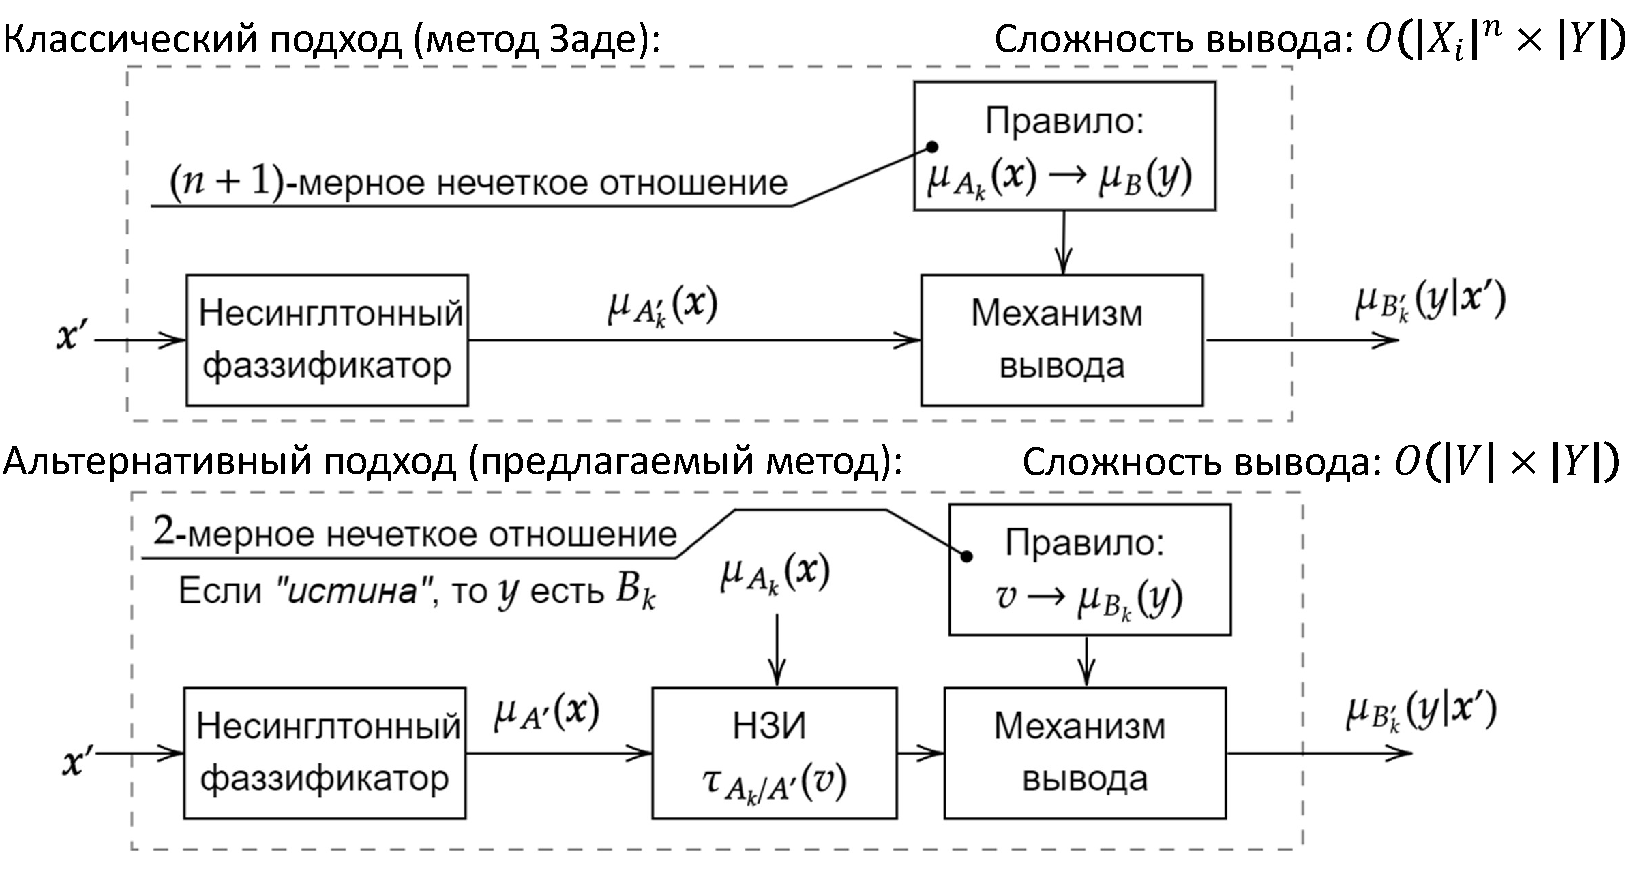
\includegraphics[scale=0.45]{ftv-schema-comparizon}
\caption{Сравнение классической схемы нечеткого вывода и схемы нечеткого вывода на основе НЗИ}
\label{fig:ftv-schema-comparizon}
\end{figure}

Порядок функции временной сложности вычисления $B'_k$ на основе выражения (\ref{eqn:ftv-compute-11}) составляет $O\left(n|V|^2+|V|\cdot |Y|\right)$, где $V=CP(A_k, A')$. Сравнение схем нечетких выводов с соответствии с соотношениями (\ref{eqn:fuz-problem-4}) и (\ref{eqn:ftv-compute-11}) представлены на рис. \cref{fig:ftv-schema-comparizon}.

\todo{\ul{Вывод типа Мамдани}}

В \cite{Sinuk2023} ослаблено ограничение на использование одной и той же $T$-нормы в формуле композиционного правила вывода в работах Менделя для случая вывода типа Мамдани, а также показано, что вывод по отдельному правилу в случае $T_2 = T_4 = T$ может быть записан через \textit{меру возможности}:
\begin{align*}
	\mu_{B'_k}(y) = \sup_{v\in[0;1]}\left\{\tau_{A_{k}|A'} \overset{\mathrm{T_2}}{\star} (v \overset{\mathrm{T_4}}{\star} \mu_{B_k}(y)) \right\} = \textstyle\prod_{\mathbf{A_k}|\mathbf{A'}} \overset{\mathrm{T}}{\star} \mu_{B_k}(y),
\end{align*}
где $\prod_{\mathbf{A_k}|\mathbf{A'}}=\sup_{v\in[0;1]}\left\{\tau_{A_{k}|A'} \overset{\mathrm{T}}{\star} v\right\}$.


Если при этом используется дефаззификация \textit{по центру сумм (CoS)} и $T$-норма Ларсена, то, как доказано в \cite{Sinuk2023}, результат дефаззификации зависит от ширины гауссовой или треугольной функции принадлежности консеквента, тогда как дефаззификация \textit{по среднему центру} учитывает только параметр центра. Например, при использовании в качестве выходной ф. п. гауссовой функции $\mu_{B_k}(y) = exp(-((y-\bar{y}_k)/\sigma_k)^2)$ формула дефаззификации имеет вид: 

\begin{equation}
	\hat{y}_{CoS} = \frac{\int_{\mathbb{Y}} y \sum_{k=1}^{N} \prod_{\mathbf{A_k}|\mathbf{A'}} \overset{\mathrm{T}_2}{\star} \mu_{B_k}(y)}{\int_{\mathbb{Y}} \sum_{k=1}^{N} \prod_{\mathbf{A_k}|\mathbf{A'}} \overset{\mathrm{T}_2}{\star} \mu_{B_k}(y)} = \frac{\sum_{k=1}^{N} \prod_{\mathbf{A_k}|\mathbf{A'}} \bar{y}_k \sigma_k}{\sum_{k=1}^{N} \prod_{\mathbf{A_k}|\mathbf{A'}} \sigma_k},
\end{equation}
поскольку $	\int_{-\inf}^{\inf}\mu_{B_k}(y) dy = \sigma_k \sqrt{\pi}$ и $\int_{-\inf}^{\inf} y \mu_{B_k}(y) dy = \bar{y}_k \sigma_k \sqrt{\pi}$.

Для предложенного метода вывода на основе нечеткого значения истинности в \cite{Karatach2024} показано, что для достаточно удаленных и непересекающихся выходных ф. п. нечетких множеств, т. е. когда $\mu_{B_k}(\bar{y}_r) = 0$ для $k \ne r$, сложность вычисления дефаззификации по центру тяжести сокращается за счет упрощения выражений импликаций:
\begin{itemize}
	\item для \textit{S}-импликации
	\begin{equation*}
		\hat{y}_{CoG} = \frac{\sum_{k=1}^{N} \overline{y}_k \Tnorm_{r=1}^N \left\{\sup_{v\in [0, 1]} \left\{\tau_{A_r|A'}\overset{\mathrm{T}_2}{\star}(1-v)\right\}\right\}}{\sum_{k=1}^{N} \Tnorm_{r=1}^N \left\{\sup_{v\in [0, 1]} \left\{\tau_{A_r|A'}\overset{\mathrm{T}_2}{\star}(1-v)\right\}\right\}},
	\end{equation*}
	\item для \textit{R}-импликации
	\begin{equation*}
		\hat{y}_{CoG} = \frac{\sum_{k=1}^{N} \overline{y}_k \Tnorm_{r=1}^N \left\{\tau_{A_r|A'}(0)\right\}}{\sum_{k=1}^{N} \Tnorm_{r=1}^N \left\{\tau_{A_r|A'}(0)\right\}},
	\end{equation*}
	\item для \textit{Q}-импликации
	\begin{equation*}
	{\fontsize{11}{6}
		\hat{y}_{CoG} = \frac{
			\sum_{k=1}^{N} \overline{y}_k \mathrm{T}_2 \left\{
			\sup_{v\in [0, 1]} \left\{\tau_{A_k|A'}\overset{\mathrm{T}_2}{\star}max(1-v, v)\right\}
			\Tnorm_{\substack{r=1\\r\ne k}}^N \left\{
			\sup_{v\in [0, 1]} \left\{\tau_{A_r|A'}\overset{\mathrm{T}_2}{\star}(1-v)\right\}
			\right\}
			\right\}
		}{
			\sum_{k=1}^{N} \mathrm{T}_2 \left\{
			\sup_{v\in [0, 1]} \left\{\tau_{A_k|A'}\overset{\mathrm{T}_2}{\star}max(1-v, v)\right\}
			\Tnorm_{\substack{r=1\\r\ne k}}^N \left\{
			\sup_{v\in [0, 1]} \left\{\tau_{A_r|A'}\overset{\mathrm{T}_2}{\star}(1-v)\right\}
			\right\}
			\right\}
		}.
	}
	\end{equation*}
\end{itemize}



\ul{Применение предложенного метода вывода в нечеткой модели для задачи классификации объектов}

Пусть производится классификация для набора объектов $\left\{q_l\right\}_{l=1}^M$, значения признаков которых значения признаков формализуются посредством термов лингвистических переменных, совокупность значений которых формирует вектор $\mathbf{x_l}=\left[x_{l1},\ldots,x_{ln}\right]$. Объекты классифицируются среди множества классов $\Omega = \left\{\omega_1, \dots, \omega_m\right\}$. Тогда база знаний нечеткой системы описывается набором из $N$ правил вида:
\begin{align*}
	R_k: \text{Если } \bigwedge_{i=1}^n \left(x_i\text{ есть }A_{ki}\right)\text{, то }\bigwedge_{j=1}^m \left(q\in\omega_j\,(\text{со степенью }\bar{z}_{kj})\right), k=\overline{1,N}.
\end{align*}
В этом правиле степень принадлежности объекта $q$ к классу $\omega_j$ задается значением $\bar{z}_{kj}$, которому можно поставить в соответствие значение лингвистической переменной $z_j$. Это значение выражается нечетким множеством имеющим в качестве базового множеств диапазон $[0,1]$, а в качестве функции принадлежности используется singleton:
\begin{equation}
\mu_{B_{kj}}(z_j) = \left\{
\begin{alignedat}{2}
	& 1, \quad & \text{eсли } z_j = \bar{z}_{kj} \\
	& 0, \quad & \text{eсли } z_j \ne \bar{z}_{kj}
\end{alignedat}
\right.
\end{equation}

Тогда при использовании дискретизированной дефаззификации по центру тяжести степень принадлежности объекта $q$ к $j$-му классу вычисляется по формуле:
\begin{align}
	\tau_{A_k|A'}(v) = \underset{i=\overline{1,n}}{\mathrm{\tilde{T}}} \left\{\mu_{CP(A_{ki}, A'_i)}(v_i)\right\}, k=\overline{1,N},\\
	\hat{z}_j = \frac{\sum_{r=1}^{N} \bar{z}_r \Tnorm_{k=1}^N \left\{\sup_{v\in [0, 1]} \left\{\tau_{\mathbf{A_k}|\mathbf{A'}}\overset{\mathrm{T}_2}{\star} I\left(v, \mu_{B_{kj}}(\bar{z}_r)\right)\right\}\right\}}{\sum_{r=1}^{N} \Tnorm_{k=1}^N \left\{\sup_{v\in [0, 1]} \left\{\tau_{\mathbf{A_k}|\mathbf{A'}}\overset{\mathrm{T}_2}{\star} I\left(v, \mu_{B_{kj}}(\bar{z}_r)\right)\right\}\right\}}.
\end{align}

%\begin{figure}[th]
%	\centering
%	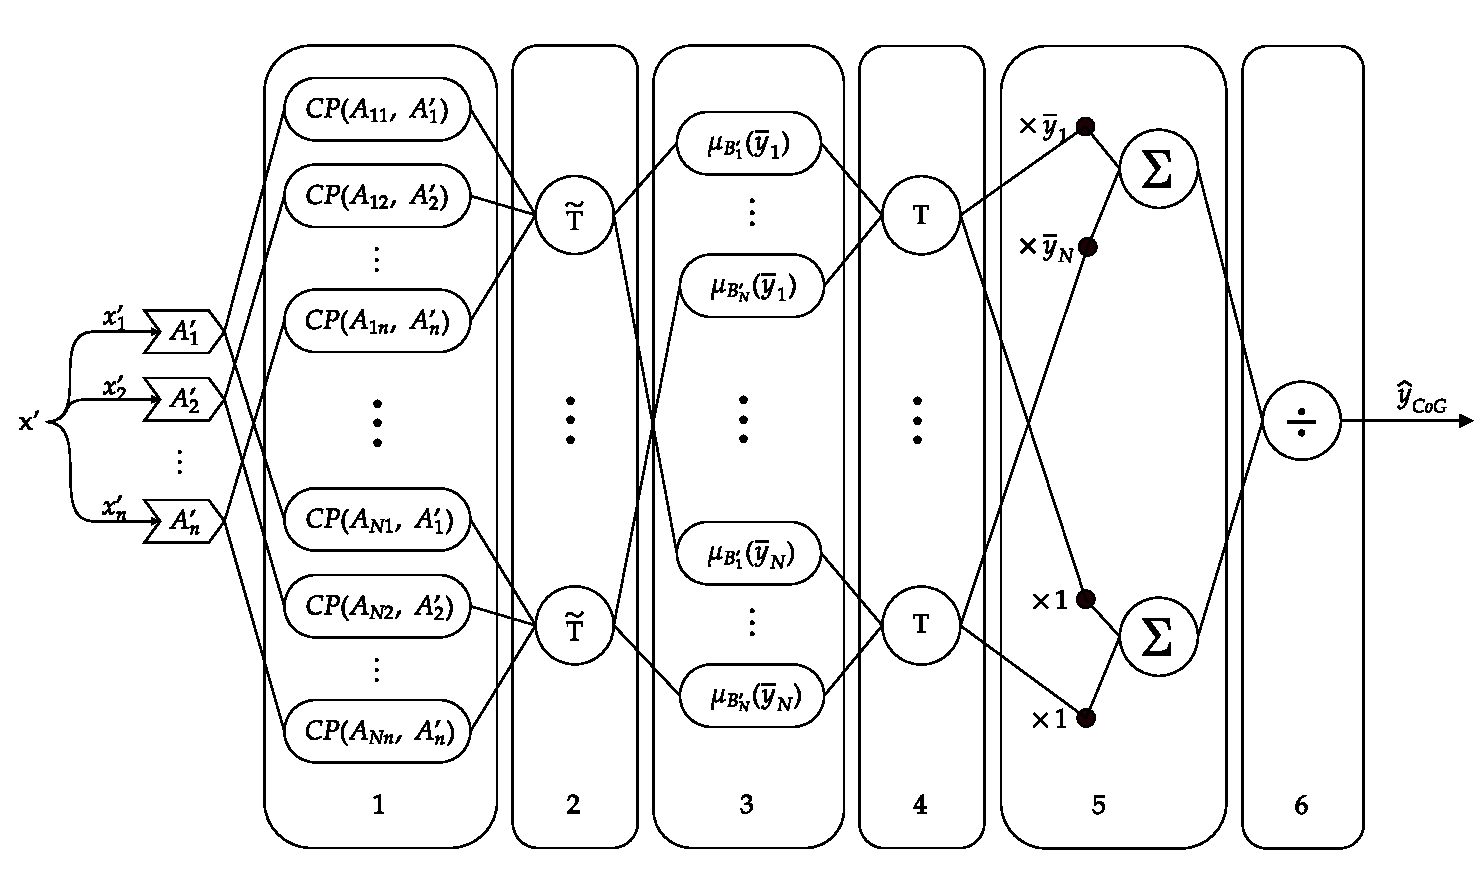
\includegraphics[scale=0.5]{neurofuzzysystem-defuzzification-cog}
%	\caption{Схема нейро-нечеткой системы с использованием дефаззификации по методу центра тяжести}
%	\label{fig:neurofuzzysystem-defuzzification-cog}
%\end{figure}



\ul{Применение предложенного метода вывода в нечеткой модели для задачи регрессии временных рядов}

Пусть задан временной ряд $\left\{y_t\right\}_{t=1}^T = \left\{y_1, \dots, y_T\right\}$, где $y_t \in \mathbb{R}$ --- измеренное значение наблюдаемой переменной в момент времени $t$, а $T$ --- длина доступной выборки. При моделировании временных последовательностей с использованием нейро-нечетких систем каждое значение $y_t\in \mathbb{Y}\subseteq \mathbb{R}$ фаззифицируется в нечеткое множество $A'_t$. Тогда для прогнозирования значения $\hat{y}_{t+h}$ с горизонтом $h$ на основании среза наблюдений $y_{t-p+1}, \dots, y_t$ можно использовать нечеткую систему с базой из $N$ правил вида:
\begin{align*}
	R_k: \text{Если } \bigwedge_{i=1}^p \left(y_{t-i+1}\text{ есть }A_{ki}\right)\text{, то }y_{t+1}\textrm{ есть }A_{k\,p+1}, k=\overline{1,N},
\end{align*}
где $p$ --- размер окна запаздывания (порядок модели, количество входов нечеткой системы).

В задаче регрессии дискретная формула дефаззификации по центру тяжести не показывает достаточной точности, а непрерывная ее формулировка имеет большую вычислительную сложность. Поэтому в работе для регрессии используется дефаззификация по среднему максимуму:

\begin{align}
	\tau_{A_k|A'}(v) = \underset{i=\overline{1,n}}{\mathrm{\tilde{T}}} \left\{\mu_{CP(A_{ki}, A'_{t-p+i})}(v_i)\right\}, k=\overline{1,N},\\
	\hat{y}_{t+h} = \argmax_{y\in\mathbb{Y}} \left\{\Tnorm_{k=1}^N \left\{\sup_{v\in [0, 1]} \left\{\tau_{\mathbf{A_k}|\mathbf{A'}}\overset{\mathrm{T}_2}{\star} I\left(v, \mu_{A_{k\,p+1}}(y)\right)\right\}\right\}\right\}.
\end{align}

\begin{figure}[thb]
	\centering
	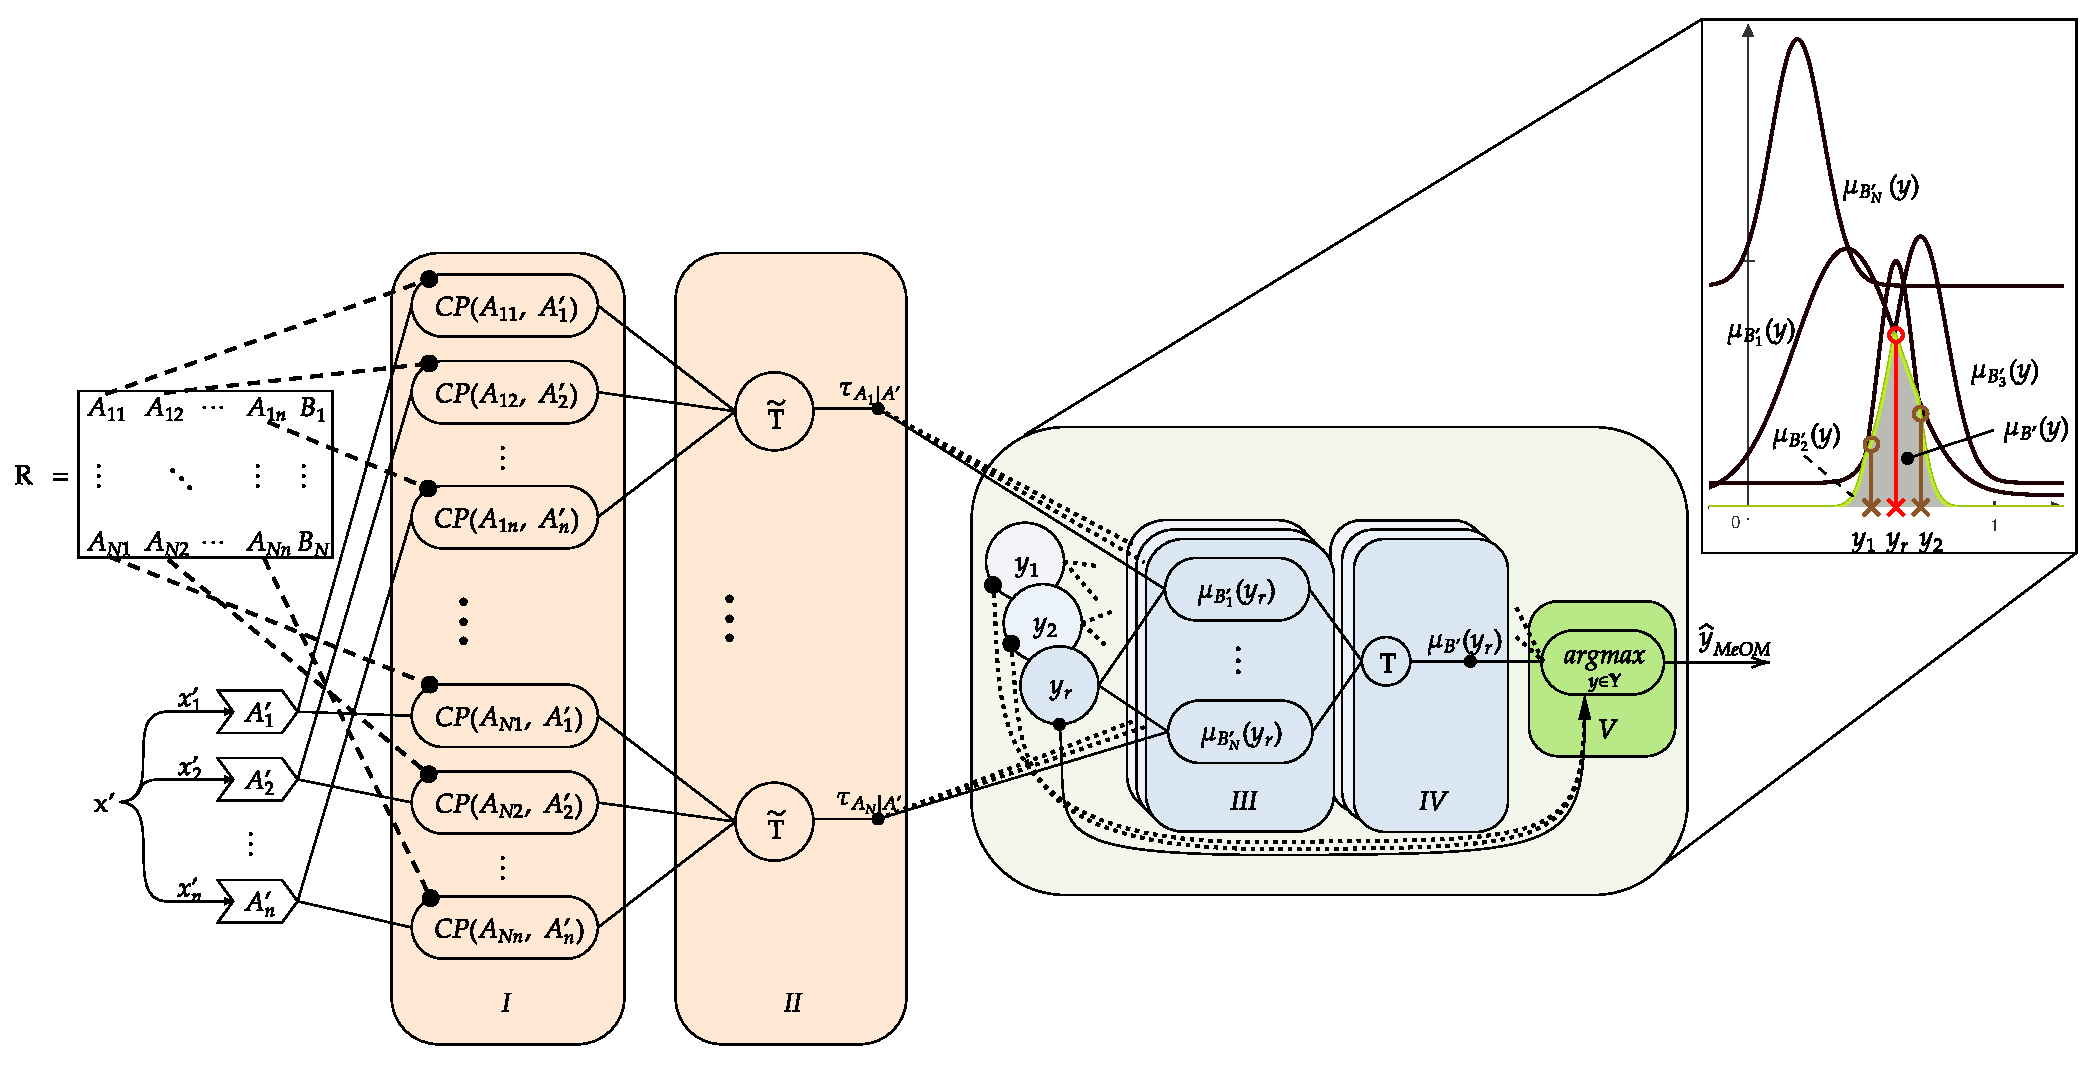
\includegraphics[width=\linewidth]{nfs-ftv-and-defuz-meom-with-defuz-demo}
	\caption{Схема нейро-нечеткой системы с вычислением НЗИ и дефаззификацией по среднему максимуму, а также пример работы дефаззификации.}
	\label{fig:nfs-ftv-and-defuz-meom-with-defuz-demo}
\end{figure}





%Нейро-сетевая структура изображена на рисунке 

%\begin{figure}[ht]
%	\centering
%	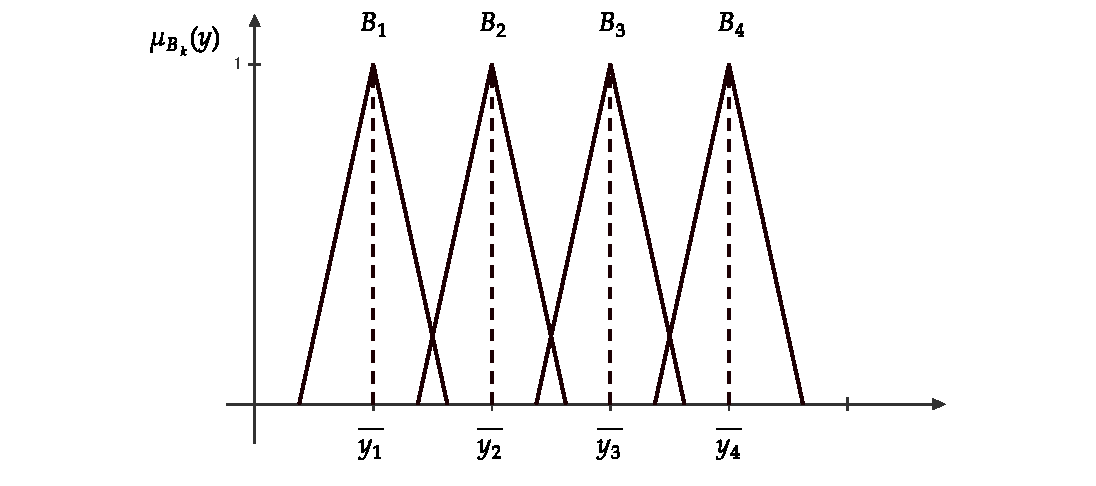
\includegraphics[scale=0.5]{out-mf-with-low-crossing}
%	\caption{Пример нечетких множеств, удовлетворяющих условию $\mu_{B_k}(y_r) = 0$ для $y \ne r$.}
%	\label{fig:out-mf-with-low-crossing}
%\end{figure}



\textbf{Третья глава} посвящена выработке эффективной параллельной реализации разработанного метода нечеткого вывода на основе нечеткого значения истинности с использованием технологии CUDA. В главе описан ключевые особенности организации вычисления нечеткого вывода при использовании технологии CUDA, параллельный алгоритм свертки НЗИ, особенности реализации методов дефаззификации в нечеткой модели регрессии и схема ускоренного вывода регрессионной нечеткой системы за счет предварительного отбора правил с ближайшими антецедентами.

\ul{Параллельный алгоритм свертки НЗИ}

При программной реализации вычисления и свертки НЗИ $\tau_{A_{ki}|A'_i}$ вычисление производится в точках расчетной сетки. \ul{Значение НЗИ по $i$-му входу в точке расчетной сетки $v_j$ в данной работе обозначается $ftv_i[v_j]$ (\textit{ftv --- fuzzy truth value}).} Расчетная сетка размера $D_{ftv}$ задается на пространстве $\mathbb{V}=[0;1]$ мощности $|\mathbb{V}|$.

Для нахождения свертки НЗИ по одному правилу можно составить алгоритм на основе формулы (\ref{eqn:ftv-compute-10}). Вычислительная сложность при параллельной реализации такого алгоритма составит $O\left(D_{ftv}^2 \cdot \log{n}\right)$. Значения $ftv_i[v_j]$ необходимо вычислить до запуска алгоритма свертки, что потребует сложности по памяти $O\left(D_{ftv}\cdot n\right)$.

\begin{algorithm}
	\begin{algorithmic}
		\Require $ftv_i,\ i=\overline{1,n}$ --- это $\tau_{A_{ki}|A'_i}$ дискретизированная в точках $v_j$
		\State $max\_ftv[i] = 0;$
		\For{$v_j = 1\dots0$}
		\State $s \gets \left\{ftv_i[v_j] \mid ftv_i[v_j] >= max\_ftv[i]\right\};$
		\State $max\_ftv[i] \gets max(max\_ftv[i], ftv_i[v_j]);$
		\State $v\_max\_index \gets \mathrm{arg\,max}_i\left\{ftv_i[v_j]\right\};$
		\If{$s = \emptyset \And i = v\_max\_index$}
		\State $r[i] \gets ftv_{i}[v_j];$
		\Else
		\State $r[i] \gets max\_ftv[i];$
		\EndIf
		\State $ftv\_reduced[v_j] \gets \underset{i}{T_3}\left\{r[i]\right\}$;
		\EndFor
		\State \Return $ftv\_reduced$
	\end{algorithmic}
	\caption{Алгоритм свертки НЗИ при $T_1=min$}
	\label{alg:ftv-reduction}
\end{algorithm}

\begin{figure}[ht]
	\centering
	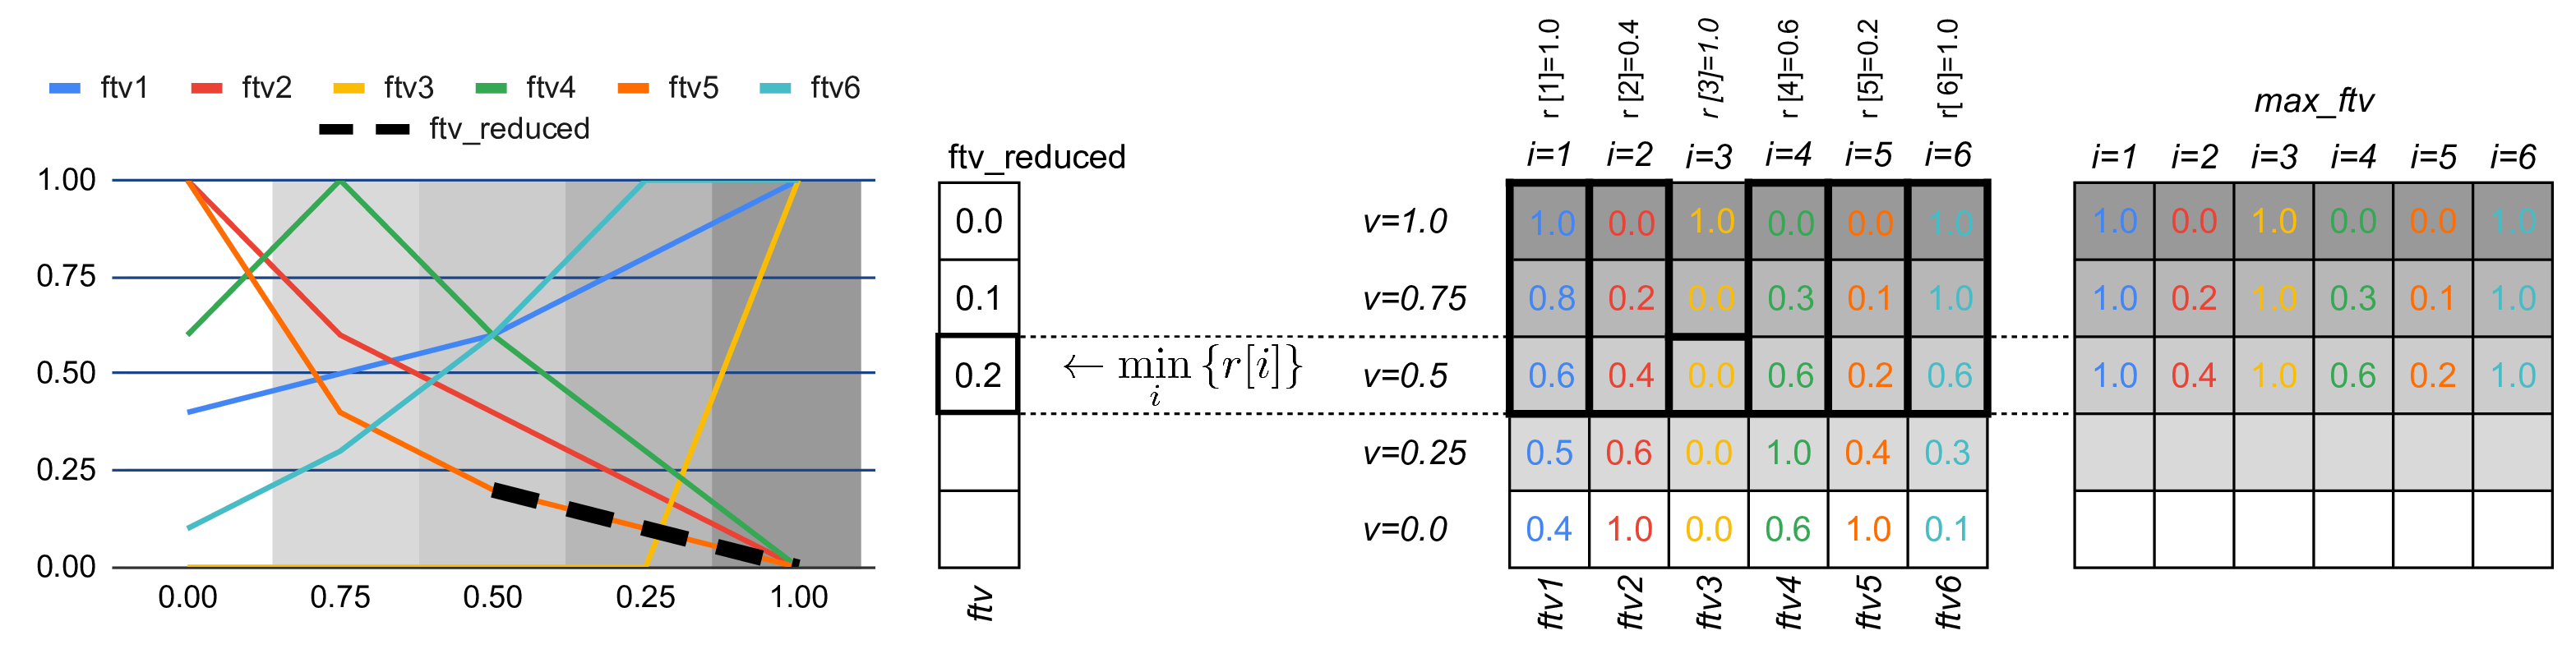
\includegraphics[width=\textwidth]{ftvs-reduction-example-gradient}
	\caption{Пример работы параллельного алгоритма свертки НЗИ при расчетной сетке состоящей из 5 точек.}
	\label{fig:ftvs-reduction-example}
\end{figure}

При выполнении работы был разработан параллельный алгоритм свертки НЗИ \cite{Karatach2023b} с вычислительной сложностью $O\left(D_{ftv}\cdot \log{n}\right)$. Алгоритм \ref{alg:ftv-reduction} разработан при допущении, что $T_1 = min$, тогда $\underset{i=\overline{1,n}}{\mathrm{T_1}}v_i = \min_{i=\overline{1,n}} v_i$ в формуле (\ref{eqn:ftv-compute-8}). При работе алгоритм итеративно продвигается от 1 к 0 в области $\mathbb{V}$, как показано на рисунке \cref{fig:ftvs-reduction-example}. На каждой $j$-й итерации вычисляются значения $ftv_i[v_j]$, которые агрегируются в одном вспомагательном массиве \textit{max\_ftv}, который требует сложности по памяти $O\left(n\right)$.

%При дискретизированном вычисление ф. п. свертки НЗИ в некоторой точке расчетной сетки $v_j\in [0,1]$ потребуется просматривать значения НЗИ в отрезке $[v_j, 1]$, то есть имеет вычислительную сложность $O(D_{ftv})$, где $D_{ftv}$ --- число точек расчетной сетки ф. п. НЗИ. Таким образом вычисление свертки НЗИ по формуле (\ref{eqn:ftv-compute-11}) может быть распараллелено по точкам расчетной сетки, а нахождение $\tau_{\mathbf{A_k}|\mathbf{A'}}(v_j)$ использует операцию свертки, которая в имеет ограниченную возможность распараллеливания, но в целом требует большого количества повторных вычислений значений $\tau_{A_{ki}|A'_i}(v_k), v_k\in [v_j, 1]$. В \ref{alg:ftv-reduction} \cite{} предложен алгоритм вычисления свертки НЗИ сразу по всем входам с использованием техники динамического программирования, имеющий линейную зависимость от размера расчетной сетки $D_{ftv}$..


\ul{Библиотека с параллельной реализацией нечеткого вывода на основе технологии CUDA}

Для более оперативного проведения экспериментов и практического применения в нагруженных промышленных приложениях была выполнена параллельная реализация нечеткого вывода на основе НЗИ с использованием языка программирования С++ и технологии CUDA. Для удобства использования к разработанному модулю вывода был реализован интерфейс из языка Python с помощью расширения Cython. Схема использования изображена на рисунке \cref{fig:application-schema-diagram}.

Важным достоинством реализации является полная организация вычислений внутри \textit{потоковых мультипроцессоров} графических ускорителей за счет размещения всей базы правил и пакета экземпляров входных данных в разделяемой памяти на чипе потокового мультипроцессора, что предотвращает возникновение простоя арифметико-логических модулей при ожидании загрузки порции данных (например, базы правил) из глобальной памяти графического ускорителя. Также, вычисления организованы внутри группы из 32 CUDA-нитей, что избавляет от необходимости синхронизации внутри CUDA-блока и позволяет использовать инструкции аппаратной свертки массивов чисел внутри таких групп.

В библиотеке реализована дискретизированная дефаззификация по центру тяжести и дефаззификация по среднему максимуму. Для точного вычисления значения дефаззификации выхода нечеткой системы для задачи регрессии используется метод оптимизации \textit{Gradient-aware Particle Swarm Optimization}.

\begin{figure}[ht]
	\centering
	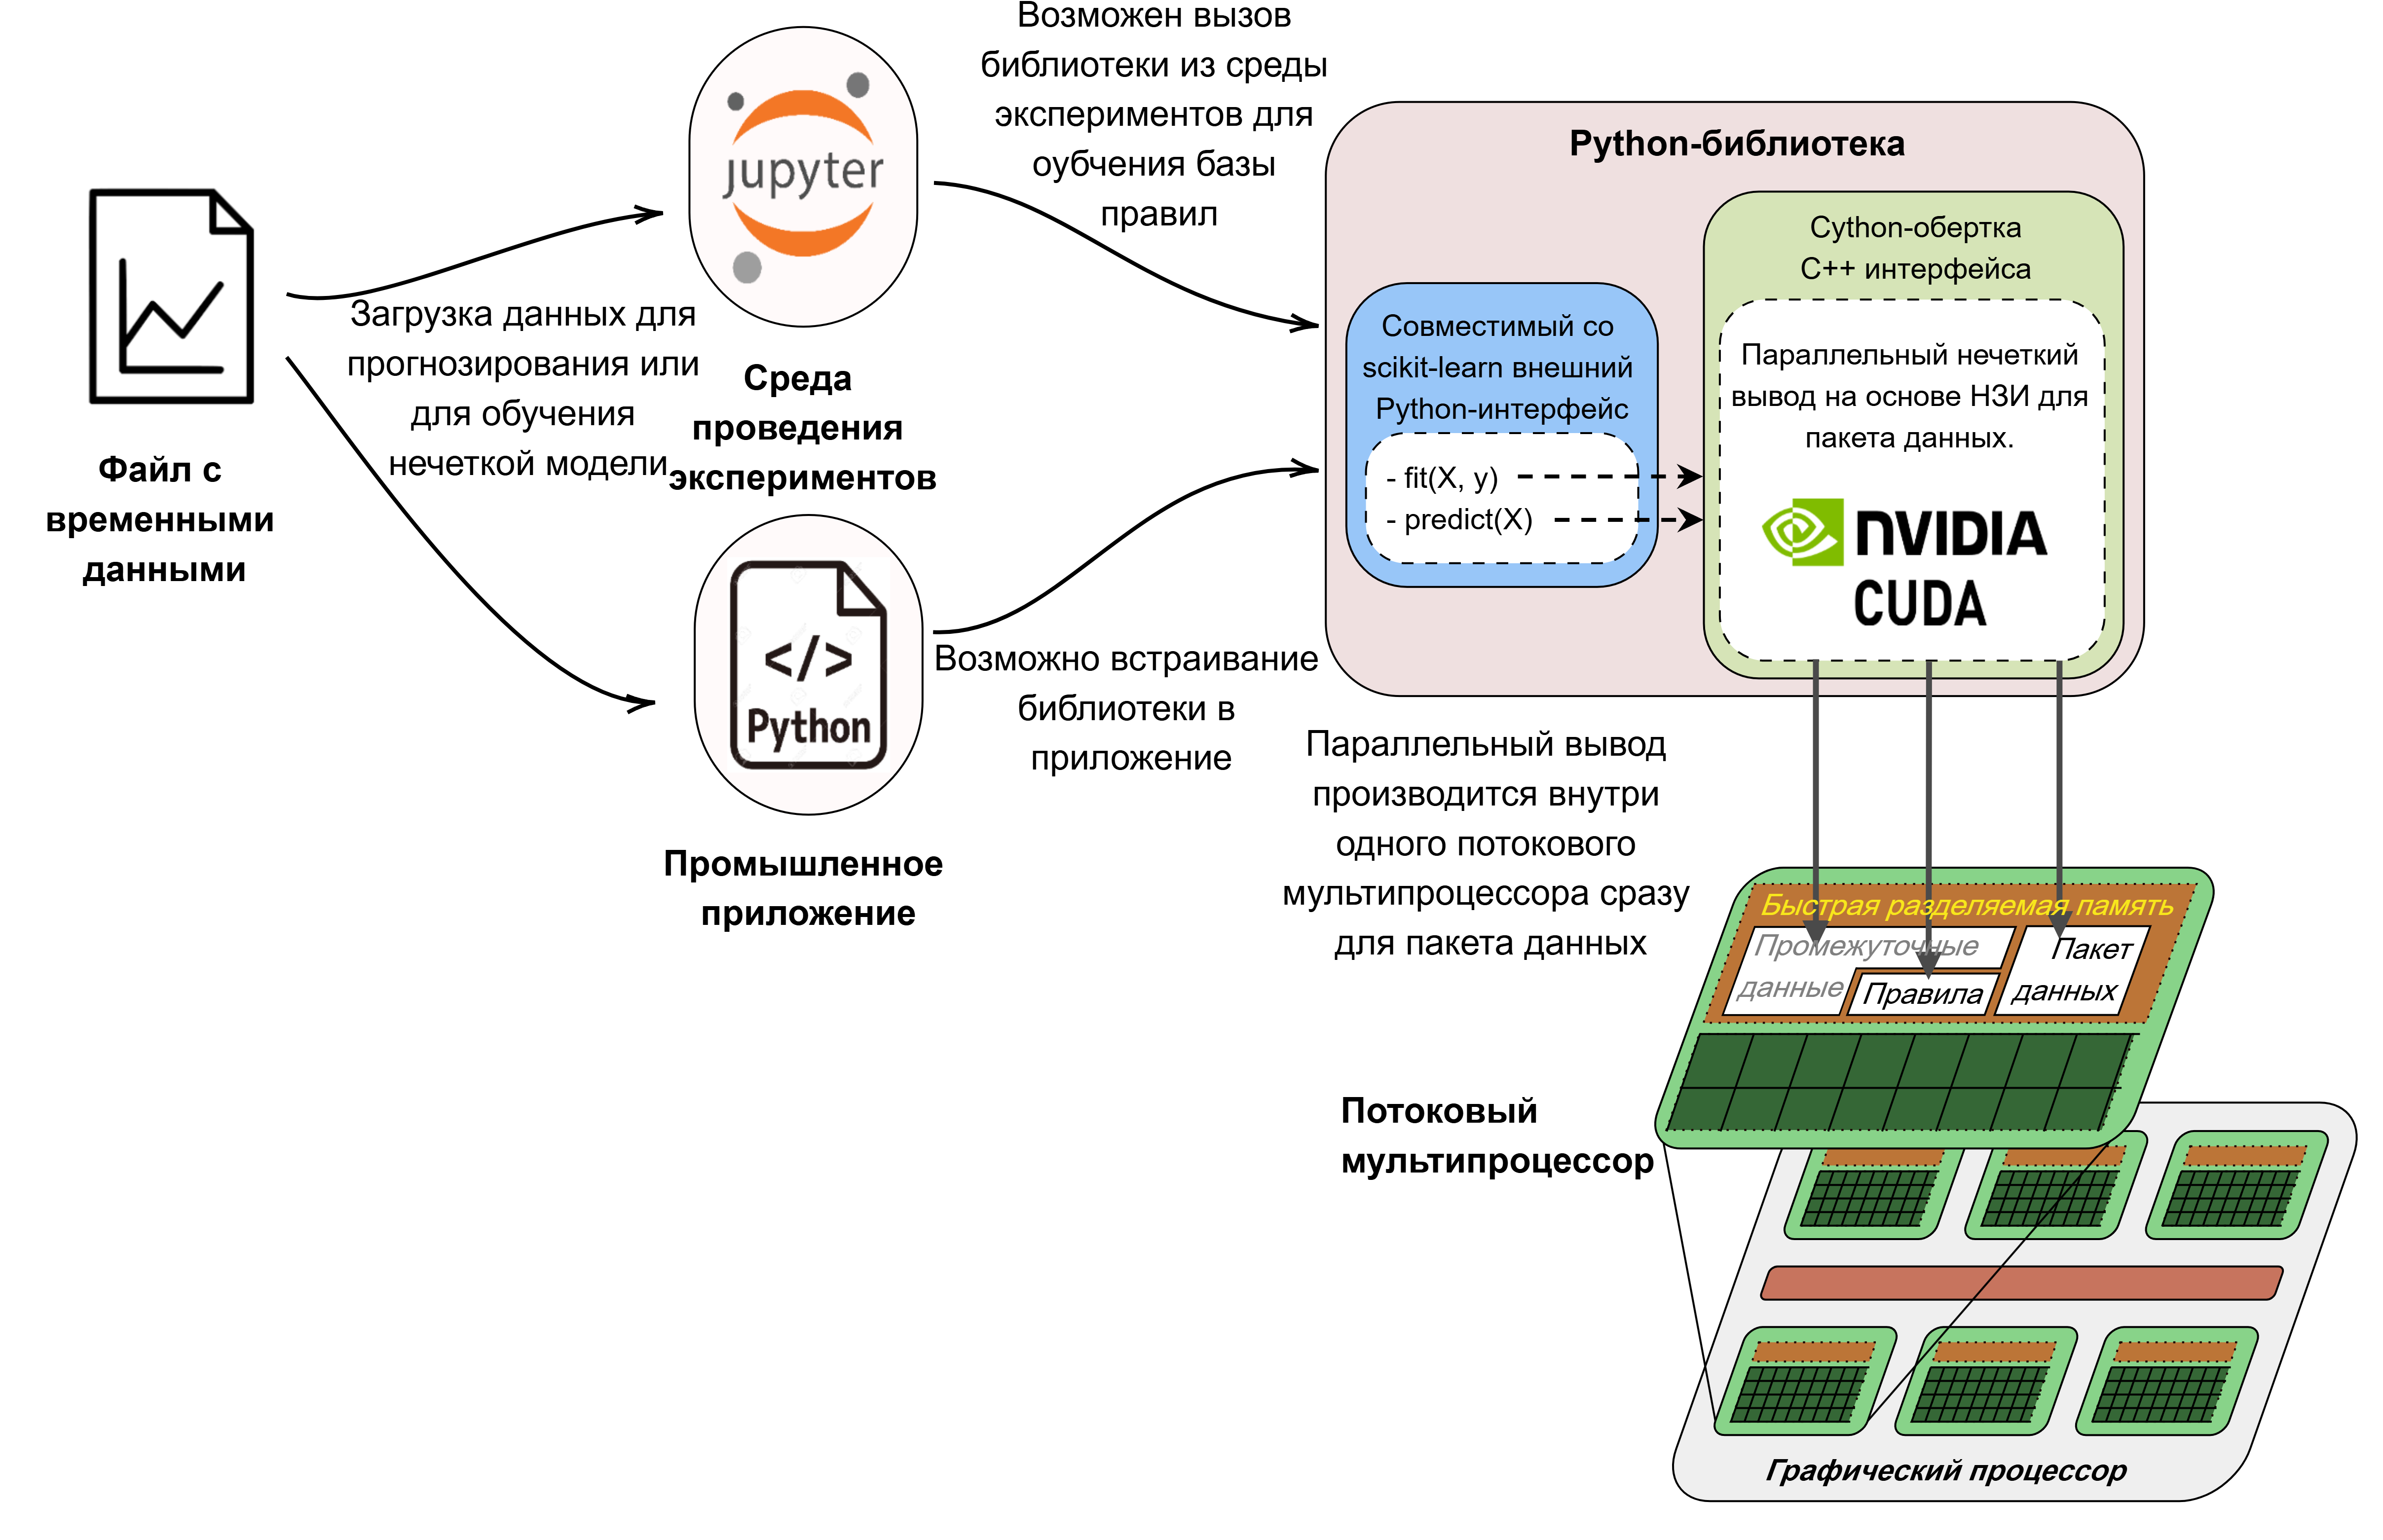
\includegraphics[width=\linewidth]{application-schema-diagram}
	\caption{Схема использования библиотеки для нечеткого моделирования и прогнозирования временных рядов.}
	\label{fig:application-schema-diagram}
\end{figure}

\textbf{Четвёртая глава} содержит описание нескольких проведенных экспериментов для оценки характеристик разработанной нечеткой модели прогнозирования временных рядов. Первый эксперимент направлен на подтверждение полиномиальной зависимости времени нечеткого вывода от количества входов нечеткой системы, а также на прирост качества прогнозирования при использовании нечеткого вывода логического типа с несинглтонной фаззификацией. Второй эксперимент был проведен для оценки качества в прикладной задаче прогнозирования временных рядов.

Первый эксперимент проводился с использованием синтетического набора данных Mackey-Glass (M-G). В данной работе этот набора данных был сгенерирован в результате решения дифференциального уравнения:
\begin{equation}
	\frac{dx(t)}{dt} = \beta\frac{x(t-\tau)}{1+x(t-\tau)^n}-\gamma x(t)
	\label{eqn:mackey-glass-definition},
\end{equation}
со значениями параметров $\tau = 30, \beta = 0.2, \gamma = 0.1$.

В эксперименте использовался участок временного ряда $t=\overline{1,1000}$, а также применялся адаптивный метод оценки зашумленности временной последовательности в каждой точке $t$ на основе экспоненциально взвешенного скользящего среднего.

\begin{figure}[ht]
	\begin{minipage}[c]{0.49\textwidth}
		\centering
		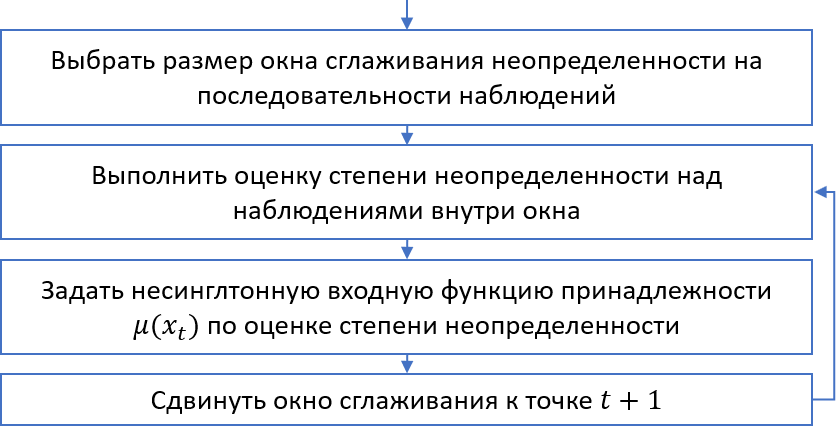
\includegraphics[width=\textwidth]{ns-procedure}
		\caption{Схема обобщенной процедуры адаптивной несинглтонной фаззификации временной последовательности.}
		\label{fig:ns-procedure}
	\end{minipage}
	\hfill
	\begin{minipage}[c]{0.49\textwidth}
		\centering
%		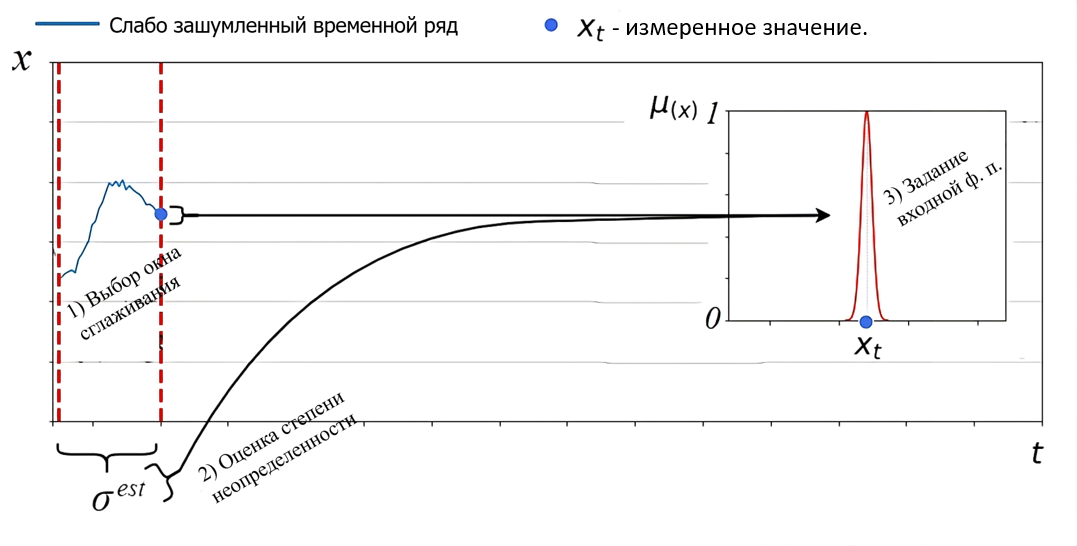
\includegraphics[width=\textwidth]{ns-demo-low-noise}
%		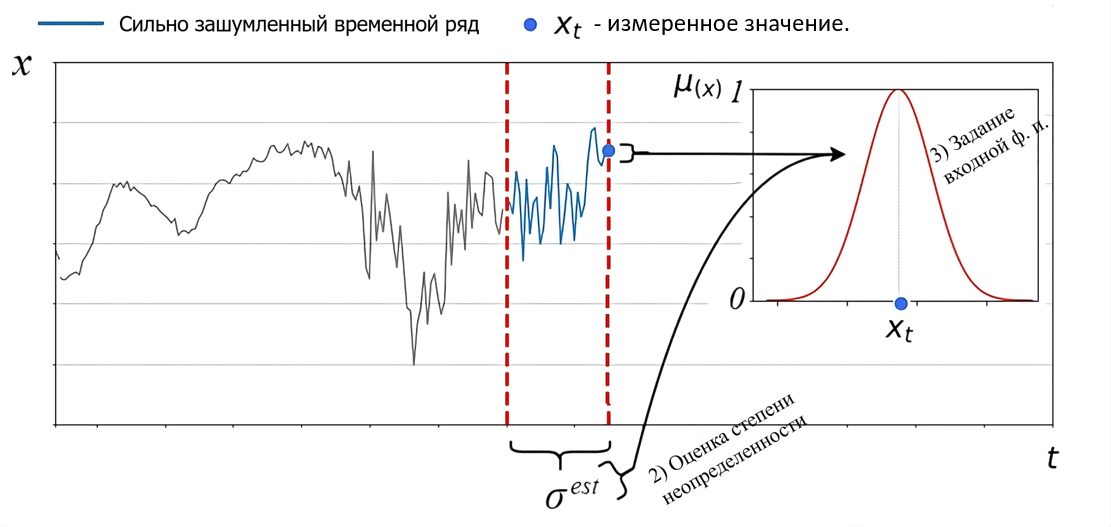
\includegraphics[width=\textwidth]{ns-demo-large-noise}
		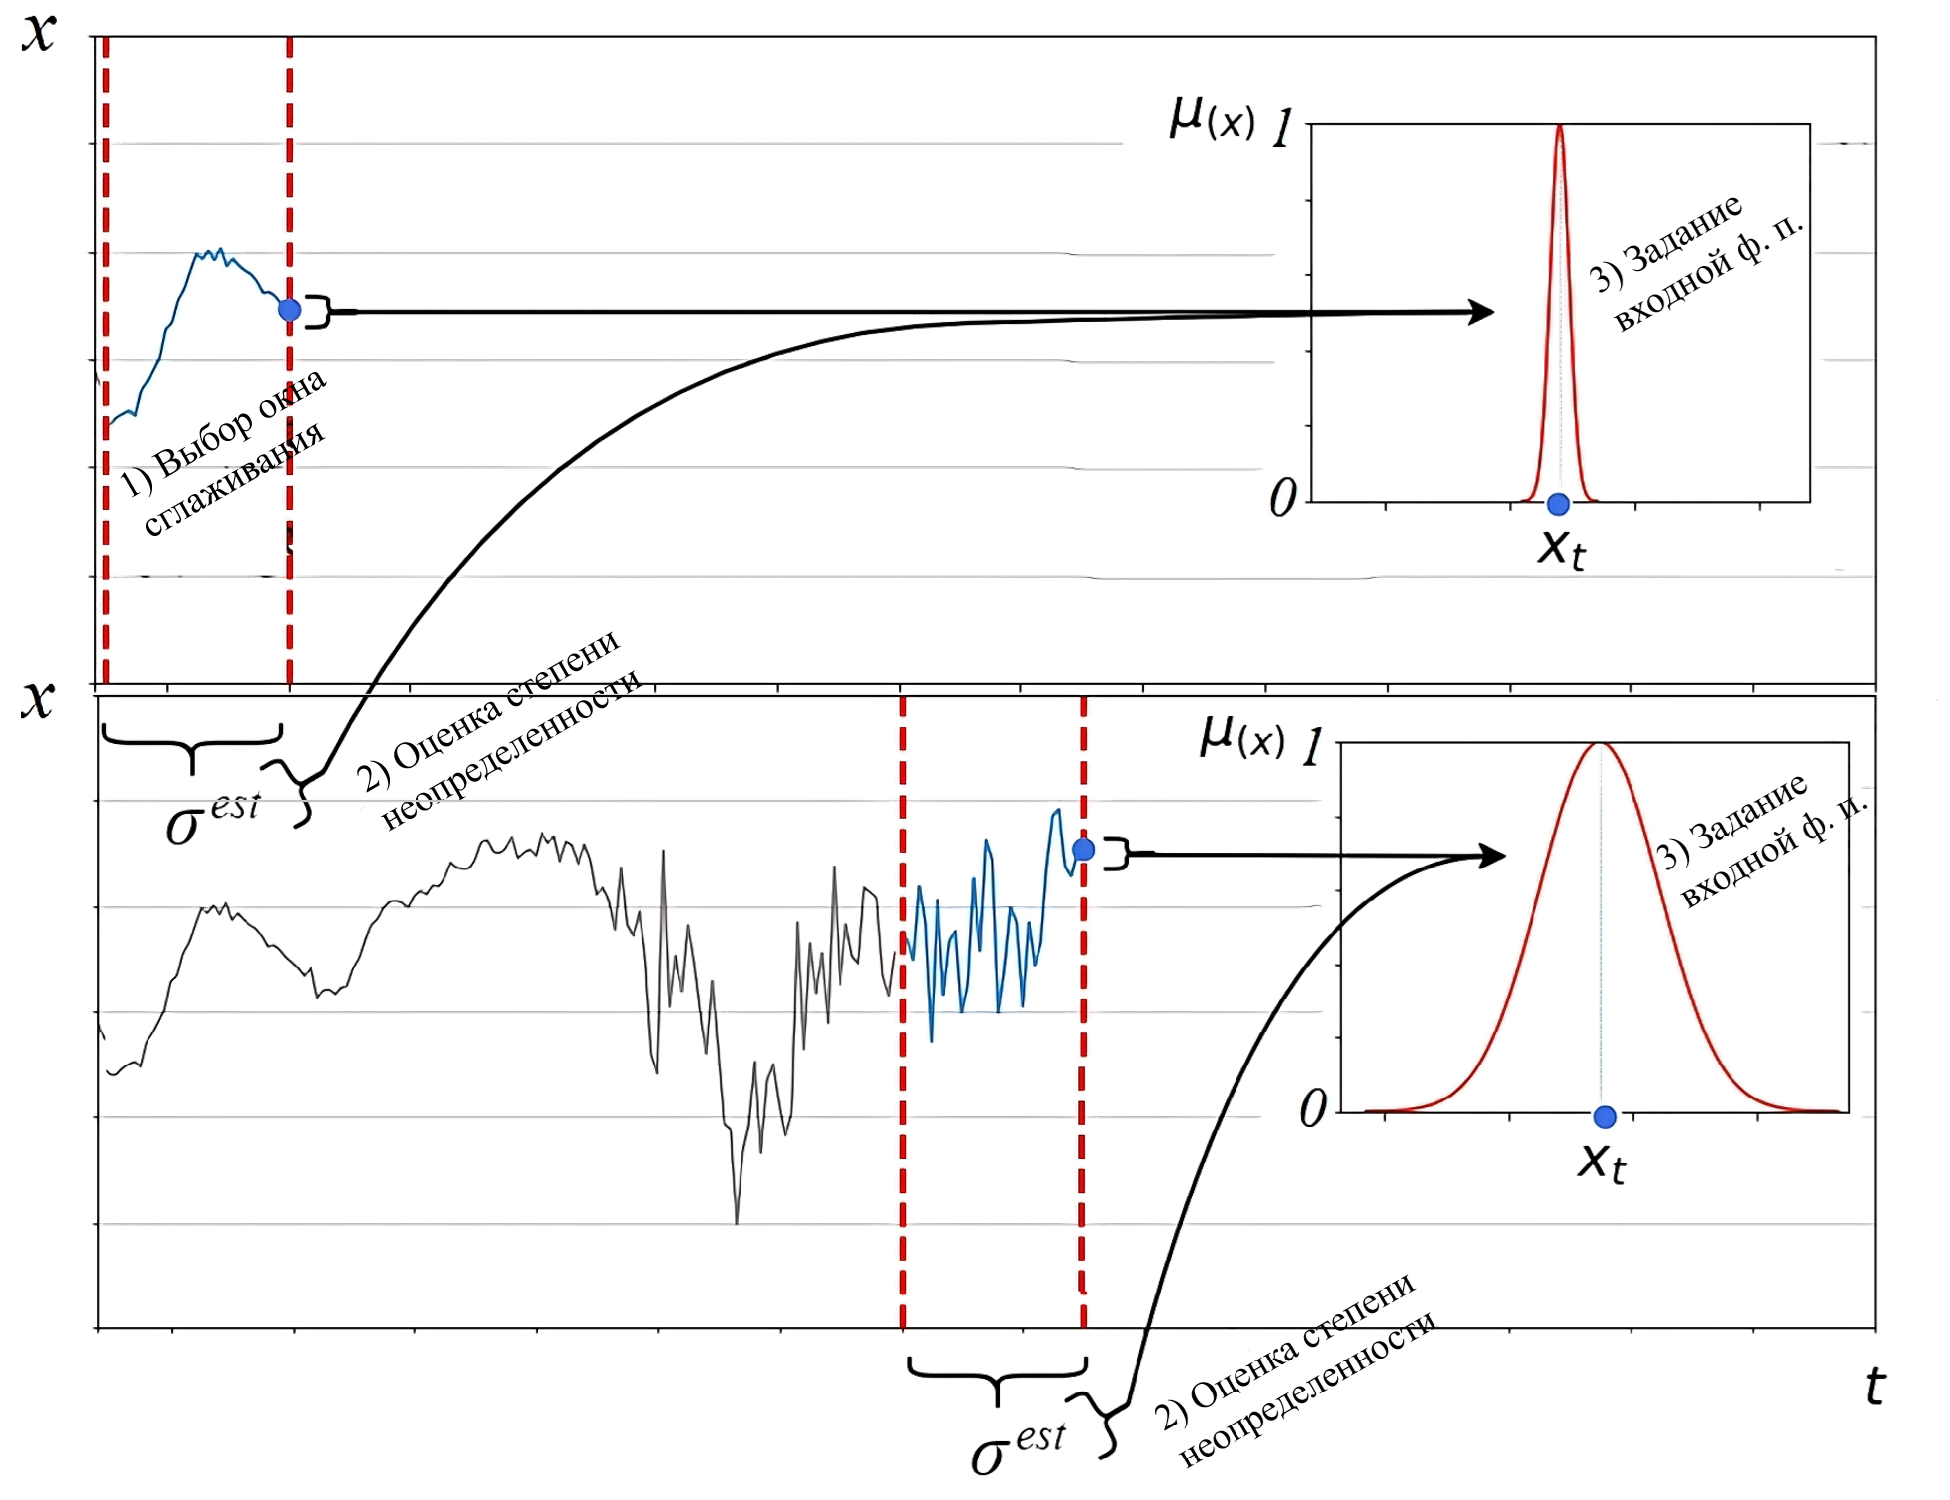
\includegraphics[width=\textwidth]{ns-demo-low-and-high-noise}
		\caption{Иллюстрация процедуры несинглтонной фаззификации временного ряда с низким (вверху) и высоким (внизу) уровнем шума.}
		\label{fig:ns-demo-low-and-high-noise}
	\end{minipage}
\end{figure}

Нечеткие множества для значений временного ряда были получены с использованием этой процедуры фаззификации временных рядов (\cref{fig:ns-procedure}) для обеспечения адаптивности оценки неопределенности в конкретной точке. Формулы для вычисления степени неопределенности показаны ниже%

\begin{minipage}{0.45\linewidth}
\begin{align}
	\label{eqn:mackey-glass-seq-diff}
	d_1 &= d_2, \notag \\
	d_t &= \frac{1}{\sqrt{2}}(x_t - x_{t-1}),
\end{align}
\begin{align}
	\hat{d}_t &= (1-\alpha) \hat{d}_{t-1} + \alpha d_t \notag \\
	&= \sum_{p=1}^t \alpha (1-\alpha)^{t-p} d_p. %\notag
	\label{eqn:mackey-glass-seq-diff-mean}
\end{align}
\end{minipage}\hfill
\begin{minipage}{0.45\linewidth}
\begin{align}
	\hat{\sigma}^2_t &= (1-\alpha) \hat{\sigma}^2_{t-1} + \alpha (d_t - \hat{d}_t) \notag \\
	&= \sum_{p=1}^t \alpha (1-\alpha)^{t-p} (d_p - \hat{d}_p)^2, \label{eqn:mackey-glass-seq-diff-var-iterative} \\
	\hat{\sigma}_t &= \sqrt{\hat{\sigma}^2_t}, \label{eqn:mackey-glass-seq-diff-std}
\end{align}
\end{minipage}

\begin{figure}[ht]
	\centering
	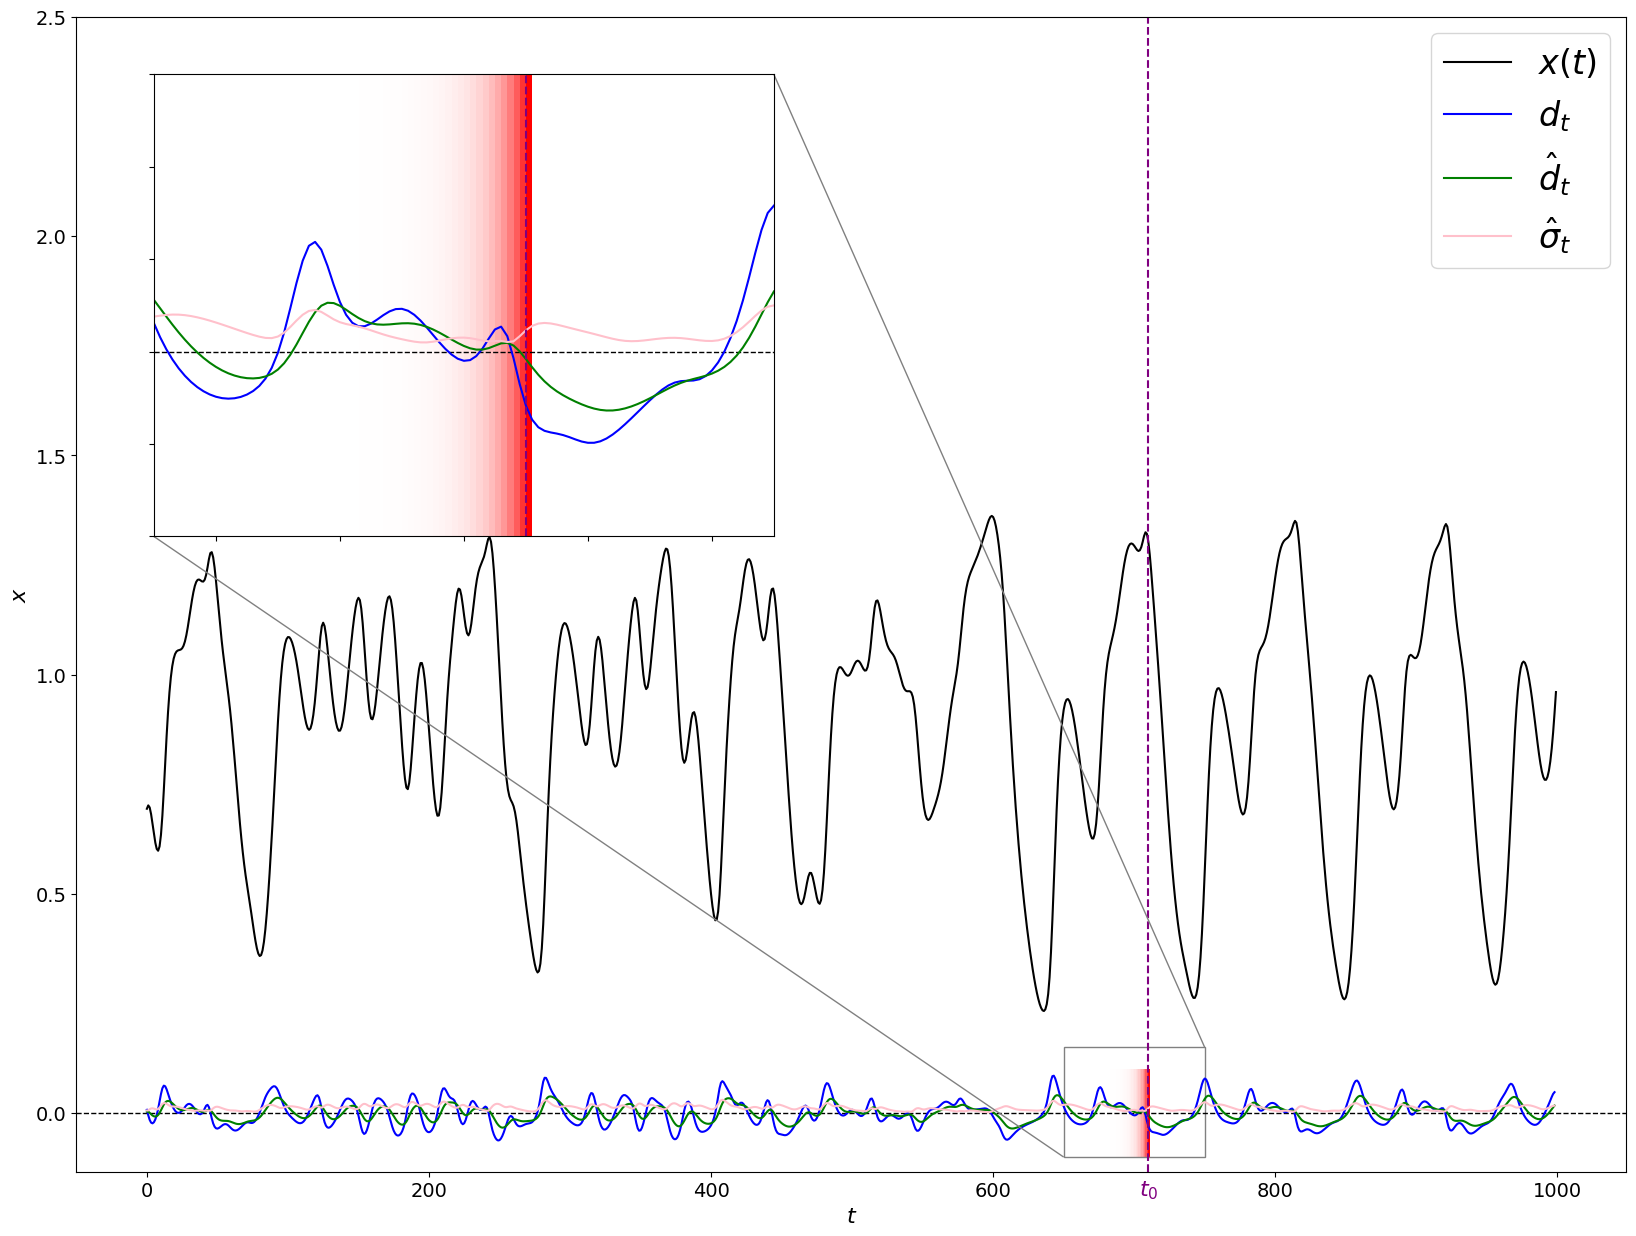
\includegraphics[scale=0.3]{mackey-glass-ewma-example}
	\caption{График сгенерированной последовательности Mackey-Glass $x(t), t\in[0;999]$, график разностей соседних точек $d_t$ последовательности $x(t)$, график $\hat{d}_t$ с наложением экспоненциально взвешенного сглаживания на последовательность разностей и график экспоненциально взвешенного скользящего среднеквадратичного отклонения разностей $\hat{\sigma}_t$. На вложенном изображении участка $t\in[650,750]$ яркостью красного цвета показано значения весового коэффициента $\alpha (1-\alpha)^{t-p}, p=\overline{1,t_0}$ при $\alpha = 0.2$.}
	\label{fig:mackey-glass-ewma-example}
\end{figure}

\begin{figure}[tbh]
	\centering
	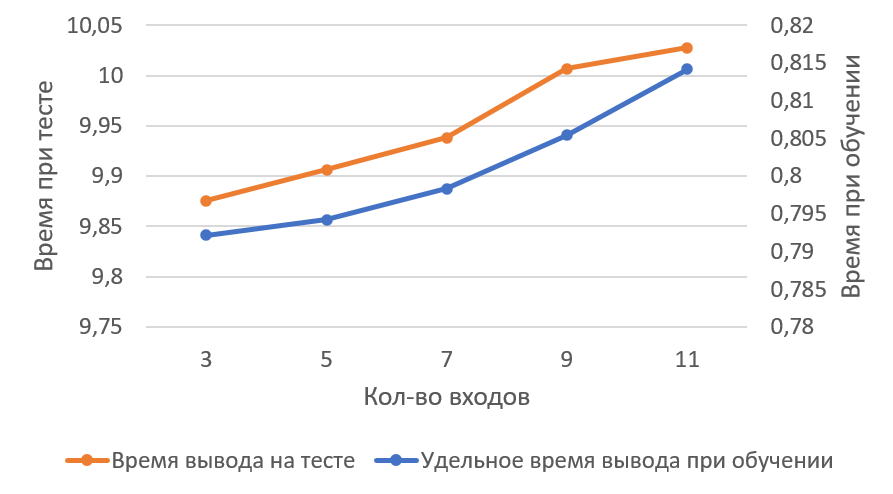
\includegraphics[scale=0.7]{mackey-glass-inference-duration}
	\caption{График длительности выполнения параллельной реализации нечеткого вывода для обучающего и тестового набора данных при количестве правил $N=30$.}
	\label{fig:mackey-glass-inference-duration}
\end{figure}

После проведенного вычислительного эксперимента были получены показатели удельного (на одну точку из набора точек одной итерации алгоритма PSO) времени работы параллельного алгоритма нечеткого вывода на основе НЗИ на обучающем наборе данных и времени работы на тренировочном наборе данных для различного размера окна запаздывания, изображенные на рисунке \cref{fig:mackey-glass-inference-duration}. На этом рисунке наблюдается линейный рост времени выполнения алгоритма с увеличением количества входов нечеткой системы, что \textbf{подтверждает утверждение о полиномиальной зависимости временной сложности метода нечеткого вывода на основе НЗИ от количества входов}.

Для сравнения с альтернативными нечеткими моделями условия этого эксперимента были выбраны такими же как в публикации \cite{}, приводящей результаты прогнозирования временного ряда M-G для нечетких систем типа Мамдани при синглтонной и несинглтонной фаззификации. Качество прогнозирования оценивалось с использованием метрики sMAPE:
\[
sMAPE = \frac{100\%}{n} \sum_{t=1}^n 
\frac{|y_t - \hat{y}_t|}{\tfrac{|y_t| + |\hat{y}_t|}{2}},
\]
где $y_t$ и $\hat{y}_t$ соответствуют истинному и предсказанному значению в момент времени $t$.

\begin{figure}
	\centering
	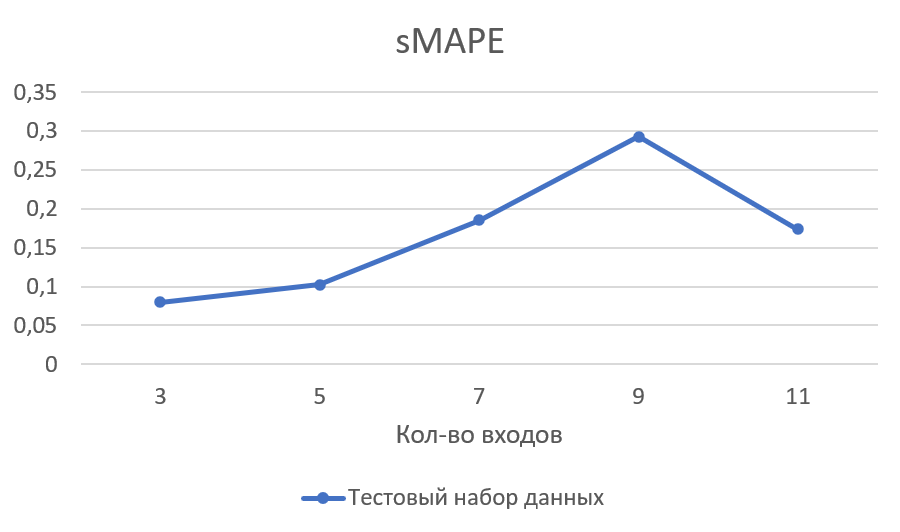
\includegraphics[scale=0.7]{mackey-glass-inference-smape}
	\caption{График значений метрики sMAPE на обучающем и тестовом наборах данных при различных размерах окна запаздывания, количестве правил --- 30.}
	\label{fig:mackey-glass-inference-smape}
\end{figure}

По итогу проведенного эксперимента лучший показатель качества прогнозирования по этой метрике на рисунке \cref{fig:mackey-glass-inference-smape} достигается при размере окна запаздывания --- 3 точки. 

%
Достигнутое в этом случае значение $sMAPE = 8\%$ при количестве правил 30, заметно превосходит точность моделирования незашумленной последовательности Mackey-Glass (M-G) с использованием синглтонной фаззификации со значением $sMAPE \approx 40\%$ в \cite{Pekaslan2020}. Также полученное качество прогнозирования сопоставимо со значением этой метрики при аналогичной конфигурации эксперимента прогнозирования временного ряда M-G в той же публикации, где для достижения точности моделирования временной последовательности $sMAPE \approx 10\%$ используется нечеткая система типа Мамдани, содержащая 184 правила\footnote{Непосредственно в самой статье не указано количество используемых правил. Однако авторами этой статьи опубликован программный код описанного в статье метода, запустив который удалось воспроизвести проводимые авторами эксперименты и восстановить количество правил в их нечетких системах.} в базе правил для не зашумленного временного ряда M-G и 597, 402, 312 правил для различных конфигураций и амплитуды добавленного шума. Данные наблюдения показывают, что \textbf{метод регрессии временных рядов на основе логического нечеткого вывода при несинглтонной фаззификации значительно превосходит качество регрессии с использованием синглтонной фаззификации, а также имеет сопоставимую с методом регрессии Мамдани при несинглтонной фаззификации точность, но при меньшем количестве правил} за счет возможности построения более сложной функции аппроксимации.

Второй эксперимент посвящен применению разработанного метода для прогнозирования помесячного объема транзакций безналичных платежей корпоративным клиентам банка. Источником неопределенности в этом наборе данных является стохастический характер динамики временной последовательности. Поэтому в этом эксперименте также использовалась процедура адаптивной несинглтонной фаззификации. В качестве метрики использовалась RMAE (relative MAE) --- отношение средней абсолютной ошибки к математическому ожиданию средних по рядам клиентов:
\[
RMAE = \frac{MAE}{\mathbb{E}[\mathbb{E}[s_t]]}.
\]

По итогу эксперимента было получено значение метрики $RMAE = 0.112/0.147$ при прогнозировании на один/три месяца соответственно. Это превосходит на $12\%/5\%$ качество прогнозирования с использованием многослойного перцептрона со значениями $RMAE = 0.128/0.157$. 




%В заключении перечислены основные научные результаты, каждый из которых подтверждён приведёнными формулами, схемами, экспериментальными графиками и таблицами: (1) формализация и аналитическая реализация метода на основе НЗИ; (2) снижение вычислительной сложности и эффективная параллельная реализация; (3) экспериментальная оценка на реальных задачах; (4) создание программной системы с поддержкой GPU и интеграцией в Python.

В \textbf{заключении} сделаны выводы о полученных в процессе работы результаты.

\pdfbookmark{Заключение}{conclusion}                                  % Закладка pdf
\section*{Заключение}
В результате выполнения работы удалось выработать метод нечеткого вывода на основе нечеткого значения истинности, позволяющий использовать тип фаззификации non-singleton при полиномиальной сложности вывода от количества входов, а также показано улучшение качества прогнозирования временных рядов с использованием логического типа вывода в сравнении с синглтонной фаззификацией и выводом типа Мамдани. В работе решены поставленные задачи и получены следующие результаты:
%% Согласно ГОСТ Р 7.0.11-2011:
%% 5.3.3 В заключении диссертации излагают итоги выполненного исследования, рекомендации, перспективы дальнейшей разработки темы.
%% 9.2.3 В заключении автореферата диссертации излагают итоги данного исследования, рекомендации и перспективы дальнейшей разработки темы.
\begin{enumerate}
  \item Анализ состояния исследований в области анализа качественных/за­шумленных данных с использованием нечеткого моделирования показал недостатки существующих методов. В частности, было выявлено отсут­ствие таких методов для моделирования систем и процессов, имеющих множество качественных/зашумленных входов, которые работали бы с полиномиальной вычислительной сложностью от количества входов и не были бы связаны со значительными упрощениями теории нечеткого логического вывода.
  \item Для логического подходов были разработаны методы, позволяющие осуществлять нечеткий логиеский вывод с полиномиаль­
  ной сложностью для произвольного набора используемых t-норм, что обеспечивает более гибкую настройку таких систем. Для определенных частных случаев в наборах используемых норм были разработаны опти­мизированные версии этих методов с использованием меры возможности.
  \item Разработан метод классификации для объектов со многими нечеткими входах\ldots
  \item Математическое моделирование показало \ldots
  \item Для выполнения поставленных задач был создан \ldots
\end{enumerate}


\pdfbookmark{Литература}{bibliography}                                % Закладка pdf
%При использовании пакета \verb!biblatex! список публикаций автора по теме
%диссертации формируется в разделе <<\publications>>\ файла
%\verb!common/characteristic.tex!  при помощи команды \verb!\nocite!

\ifdefmacro{\microtypesetup}{\microtypesetup{protrusion=false}}{} % не рекомендуется применять пакет микротипографики к автоматически генерируемому списку литературы
\urlstyle{rm}                               % ссылки URL обычным шрифтом
\ifnumequal{\value{bibliosel}}{0}{% Встроенная реализация с загрузкой файла через движок bibtex8
	\renewcommand{\bibname}{\large \bibtitleauthor}
	\nocite{*}
	\insertbiblioauthor           % Подключаем Bib-базы
	%\insertbiblioexternal   % !!! bibtex не умеет работать с несколькими библиографиями !!!
}{% Реализация пакетом biblatex через движок biber
	% Цитирования.
	%  * Порядок перечисления определяет порядок в библиографии (только внутри подраздела, если `\insertbiblioauthorgrouped`).
	%  * Если не соблюдать порядок "как для \printbibliography", нумерация в `\insertbiblioauthor` будет кривой.
	%  * Если цитировать каждый источник отдельной командой --- найти некоторые ошибки будет проще.
	%
	
	
	\ifnumgreater{\value{usefootcite}}{0}{
		\begin{refcontext}[labelprefix={}]
			\ifnum \value{bibgrouped}>0
			\insertbiblioauthorgrouped    % Вывод всех работ автора, сгруппированных по источникам
			\else
			\insertbiblioauthor      % Вывод всех работ автора
			\fi
		\end{refcontext}
	}{
		\ifnum \totvalue{citeexternal}>0
		\begin{refcontext}[labelprefix=A]
			\ifnum \value{bibgrouped}>0
			\insertbiblioauthorgrouped    % Вывод всех работ автора, сгруппированных по источникам
			\else
			\insertbiblioauthor      % Вывод всех работ автора
			\fi
		\end{refcontext}
		\else
		\ifnum \value{bibgrouped}>0
		\insertbiblioauthorgrouped    % Вывод всех работ автора, сгруппированных по источникам
		\else
		\insertbiblioauthor      % Вывод всех работ автора
		\fi
		\fi
		%  \insertbiblioauthorimportant  % Вывод наиболее значимых работ автора (определяется в файле characteristic во второй section)
		\begin{refcontext}[labelprefix={}]
			\insertbiblioexternal            % Вывод списка литературы, на которую ссылались в тексте автореферата
		\end{refcontext}
		% Невидимый библиографический список для подсчёта количества внешних публикаций
		% Используется, чтобы убрать приставку "А" у работ автора, если в автореферате нет
		% цитирований внешних источников.
		\printbibliography[heading=nobibheading, section=0, env=countexternal, keyword=biblioexternal, resetnumbers=true]%
	}
	\clearpage
}
\ifdefmacro{\microtypesetup}{\microtypesetup{protrusion=true}}{}
\urlstyle{tt}                               % возвращаем установки шрифта ссылок URL
